\documentclass{article}
\usepackage[preprint]{neurips_data_2024}
\makeatletter\renewcommand{\@noticestring}{}\makeatother % no conference/preprint notice at the bottom of page 1
\usepackage[utf8]{inputenc}
\usepackage[T1]{fontenc}
\usepackage{hyperref}
\usepackage{url}
\usepackage{booktabs}
\usepackage{amsfonts}
\usepackage{amsmath}
\usepackage{nicefrac}
\usepackage{microtype}
\usepackage{xcolor}
\usepackage{graphicx}
\usepackage{array}
\usepackage{float}
\graphicspath{{../figures/}}
\setlength{\parskip}{3pt}
\newcommand{\fig}[3][\linewidth]{\begin{figure}[!htbp]\centering\includegraphics[width=#1]{#2}\caption{#3}\end{figure}}

\title{Exploring NYC Taxi Trips: Time Patterns, Location Hotspots, Airport Travel Times and Dimensionality Reduction}

\author{%
  Emmanuel Azubuike \\
  Student number: 2698752 \\
  University of the Witwatersrand
  \And
  George Ayensu \\
  Student number: 2722188 \\
  University of the Witwatersrand
  \And
  Banele Mkhize \\
  Student number: 2663814 \\
  University of the Witwatersrand
  \AND
  COMS4060A/7056A -- Assignment 2
}

\begin{document}
\maketitle

\begin{abstract}
We analyse the 1\,458\,644 trips of the Kaggle \emph{NYC Taxi Trip Duration} training set (January--June 2016). After removing 1.4\,\% of the trips as errors (impossible passenger counts, coordinates outside New York, durations below one minute or above three hours, near-zero distances and implausible speeds), we generate distance, speed and calendar features and study (i) time patterns, (ii) spatial patterns with heat-maps and DBSCAN hotspots, (iii) travel times from the Empire State Building to JFK and Newark, and (iv) the structure of a 20\,000-trip sample with PCA, t-SNE and UMAP. Demand peaks on Friday and Saturday (statistically tied) and at 18:00--21:00 on weekdays; only Memorial Day changes the daily volume significantly. Hotspots are compact street corners that differ between Friday night (downtown nightlife) and Thursday evening (airports and Midtown hubs). A trip to JFK takes a median 46 min (about 60 min in the afternoon rush, 29 min at night) against 33 min to Newark. Non-linear embeddings reveal seven day-of-week groups and separate airport groups that PCA does not resolve; their clusters are recoverable from the original features (96\,\% kNN accuracy) but are not separated there, and their number, size and arrangement depend on the seed and hyper-parameters.
\end{abstract}

\section*{Overview and reproducibility}
All code, with the question numbers marked, is in the accompanying Jupyter notebook \texttt{DVE\_Assignment\_2.ipynb}; every figure below is produced by it. We use a fixed seed (42) throughout. The Winter Storm of 23--25 January 2016 (only 1\,614 trips on Saturday 23 January against about 8\,600 on a normal Saturday) is excluded from ``typical-day'' baselines in Sections~3 and~4. Hand-entered landmark coordinates are used only to \emph{describe} patterns and are approximate.

%====================================================================
\section{Data cleaning}
We computed the great-circle (haversine) distance between pickup and dropoff and the average speed (distance divided by duration); note that haversine is a lower bound on the road distance, so thresholds are generous. Figures~\ref{fig:q1a}--\ref{fig:q1b} show the raw data and Table~\ref{tab:funnel} the effect of each rule. The audit found no missing values, no duplicate ids and that \texttt{trip\_duration} equals dropoff $-$ pickup time for every row.

\begin{itemize}\setlength\itemsep{1pt}
\item \textbf{Passenger count} $\notin[1,6]$: zero passengers is not a paid trip and 7--9 exceed any taxi's capacity (driver-entered errors).
\item \textbf{Location}: the raw coordinates reach longitude $-121.9$, latitude $51.9$ (west coast, Canada, Atlantic). We keep trips whose pickup \emph{and} dropoff lie in lon $[-74.30,-73.65]$, lat $[40.49,40.92]$, which covers all five boroughs plus JFK and Newark.
\item \textbf{Duration} $<60$\,s (cancelled/accidental meter starts; 1\,984 trips are shorter than 10 s) and $>3$\,h (meter left running; up to 40.8 days).
\item \textbf{Distance} $<100$\,m: below GPS accuracy in Manhattan's urban canyons; the trip did not go anywhere and the speed is undefined.
\item \textbf{Speed} $>100$\,km/h (physically impossible as an \emph{average} in a city, even allowing for haversine's under-estimate) and $<1$\,km/h (slower than walking, i.e.\ a stationary vehicle with the meter running).
\end{itemize}

\fig{q1_geo_raw}{Raw pickups: world-spanning outliers (left) versus the NYC window (right, log density).\label{fig:q1a}}
\begin{figure}[!htbp]\centering
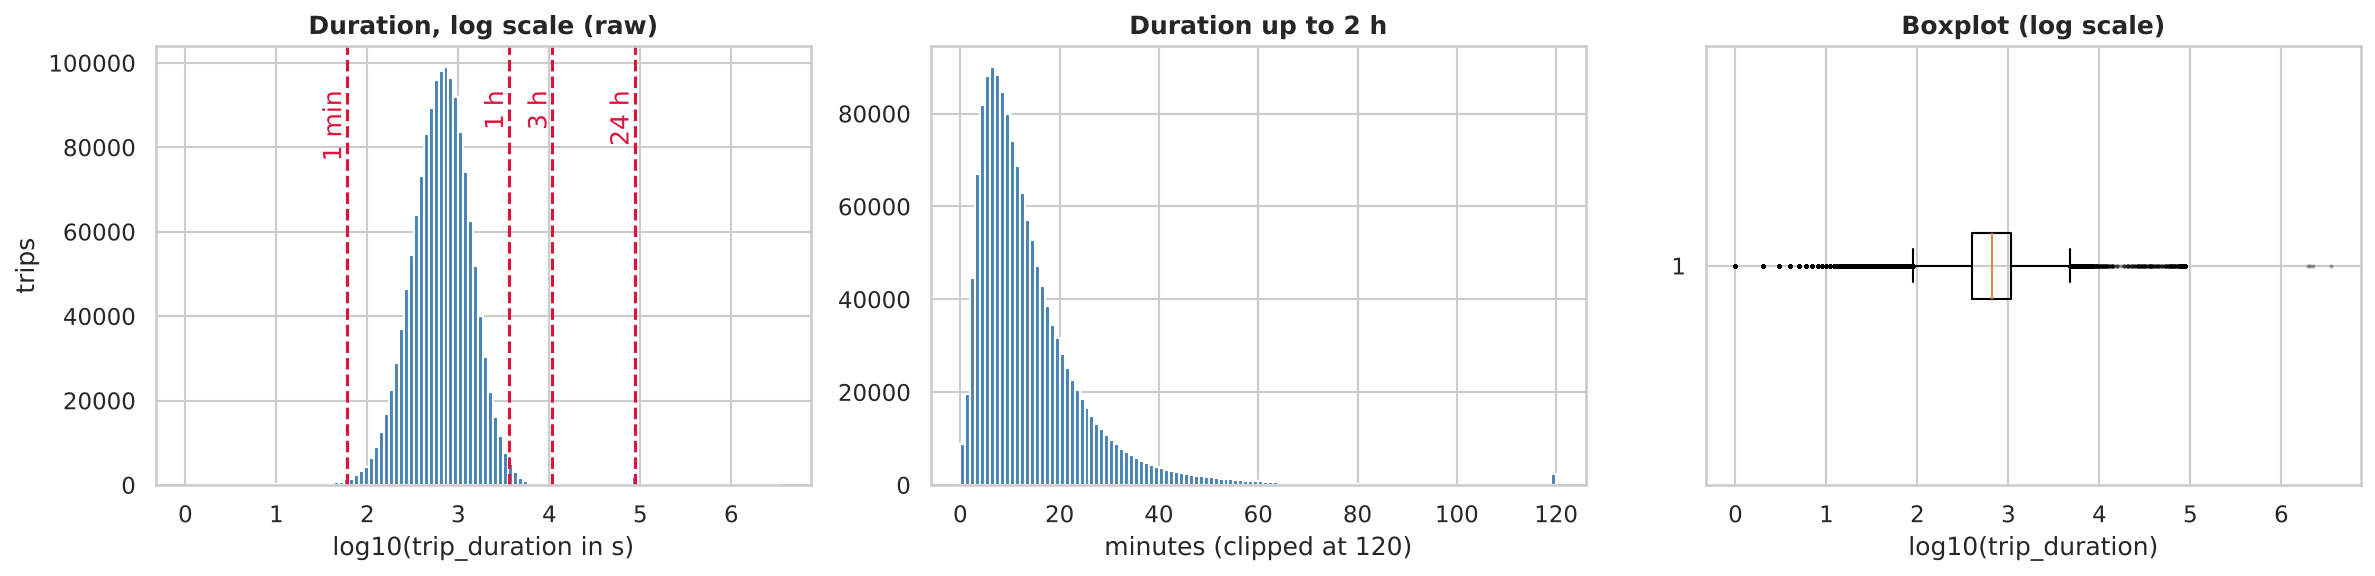
\includegraphics[width=\linewidth]{q1_duration_raw}\\[2pt]
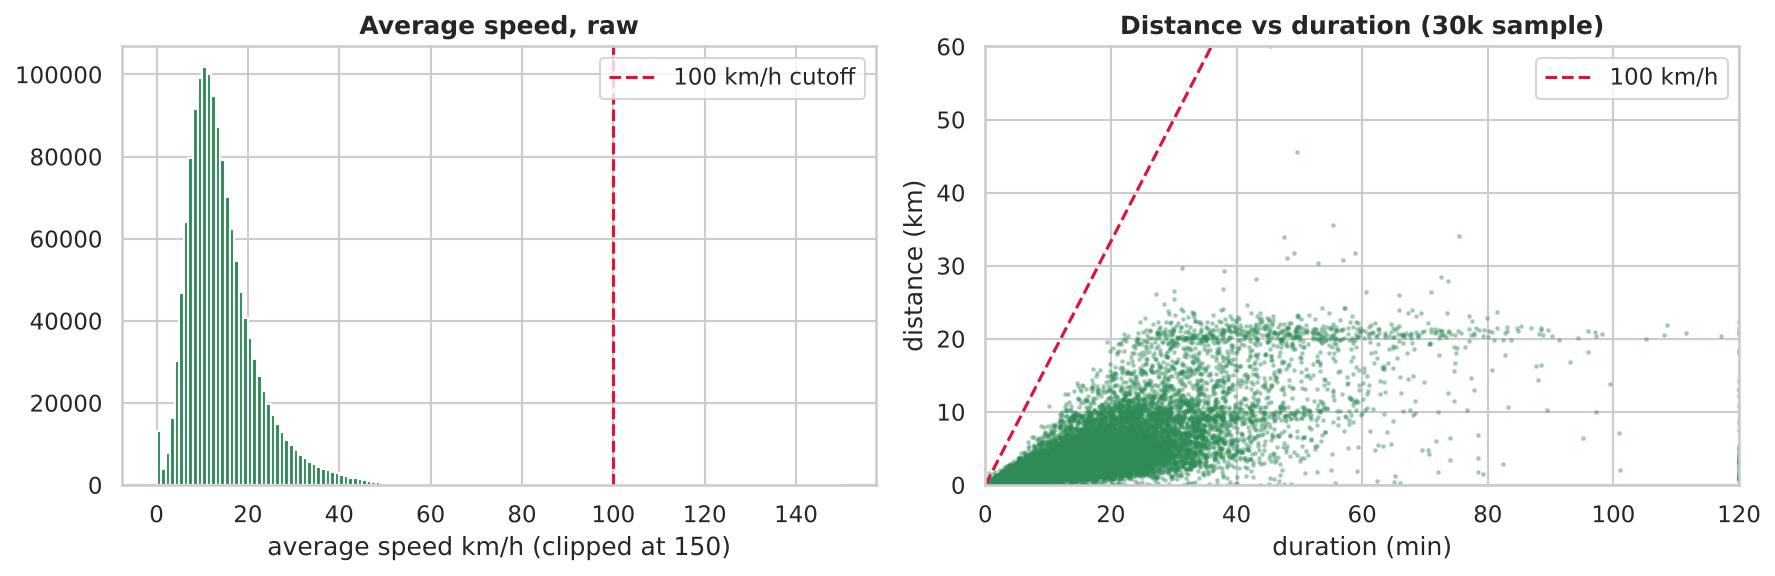
\includegraphics[width=\linewidth]{q1_speed_raw}
\caption{Raw duration (log scale) and average speed; red dashed lines are our cut-offs.}\label{fig:q1b}
\end{figure}

\begin{table}[!htbp]\centering\small
\caption{Cleaning funnel. ``Flagged'' = trips breaking the rule on its own; ``removed'' = additionally removed when rules are applied in this order. In total 20\,448 trips (1.40\,\%) are removed, leaving 1\,438\,196.}\label{tab:funnel}
\begin{tabular}{lrr}\toprule Rule & Flagged & Removed (sequential)\\\midrule
passenger count not in $[1,6]$ & 65 & 65\\
coordinates outside NYC window & 1\,096 & 1\,095\\
duration $<60$ s & 8\,595 & 8\,401\\
duration $>3$ h & 2\,112 & 2\,104\\
distance $<100$ m & 13\,319 & 7\,442\\
speed $>100$ km/h & 175 & 33\\
speed $<1$ km/h & 13\,241 & 1\,308\\\bottomrule\end{tabular}
\end{table}

\section{Feature generation}
Besides the three required features -- \textbf{distance of trip} (haversine, km), \textbf{day of week} and \textbf{average speed} (km/h) -- we generated pickup hour, date, month, weekend flag, duration in minutes, the cyclic hour encoding $(\sin\frac{2\pi h}{24},\cos\frac{2\pi h}{24})$, a Manhattan-grid ($L_1$) distance (median 1.33$\times$ the straight-line distance, as expected on a street grid), the initial compass bearing, and the distances of the pickup and dropoff to the city centre $(40.716662,-74.009899)$. The cleaned data have median distance 2.12 km, median duration 11.1 min and median speed 12.9 km/h.

%====================================================================
\section{Time-based analysis}
The data cover 182 days, so each weekday occurs exactly 26 times and weekday totals are directly comparable.

\subsection{Most popular day of the week}
\textbf{Friday and Saturday are the two busiest days and are statistically tied.} Friday has the highest total (220\,378 pickups), followed by Saturday (217\,740), Thursday (215\,509), Wednesday (207\,384), Tuesday (199\,969), Sunday (192\,396) and Monday (184\,820, the quietest; Friday is 19\,\% busier). However, the blizzard fell on a Saturday/Sunday; excluding 23--25 January, Saturday leads (8\,645 vs 8\,476 trips per day) and a Welch $t$-test on daily counts gives $p=0.37$, so the difference is not significant. Friday is among the three busiest days in all six months. Thursday--Saturday are the going-out days on top of the commute, whereas Sunday and Monday lack a strong leisure or start-of-week demand.
\fig{q3_1_popular_day}{Total pickups per weekday, distribution of daily counts (the blizzard is the outlier), and mean daily trips by month and weekday.}

\subsection{Most popular hour on each day}
Table~\ref{tab:peak} and Figure~\ref{fig:hours} show the hourly profile. Weekdays share one shape: an almost empty night (minimum 03:00--04:00), a steep rise at 06:00--08:00 (commute), a plateau, and a maximum in the evening (18:00 Mon/Tue, 19:00 Wed/Fri, 21:00 Thu: commute plus dinner and going out, shifted later as the week's going-out period begins). Saturday and Sunday have no commuter peak: demand grows through the late morning to a broad afternoon plateau and peaks at 23:00 (Saturday) and 00:00 (Sunday), i.e.\ Friday and Saturday nights spilling past midnight. Weekend nights are much busier (the quietest hour on Fri/Sat/Sun still has 76--87 pickups, against 38--52 on Mon--Thu). Plausible reasons are commuting, dinner/theatre/bar traffic with 4 a.m.\ closing times driving rides home, and the dip at about 16:00 followed by a jump at 17:00 which is consistent with the taxi shift change (day drivers hand over at 16:00--17:00); between 03:00 and 05:00 only airport runs and shift workers travel.
\begin{table}[!htbp]\centering\small
\caption{Most popular and quietest pickup hour by weekday (mean trips per hour, storm excluded).}\label{tab:peak}
\begin{tabular}{lcccccccc}\toprule & Mon & Tue & Wed & Thu & Fri & Sat & Sun\\\midrule
Peak hour & 18 & 18 & 19 & 21 & 19 & 23 & 0\\ Trips in peak hour & 495 & 512 & 521 & 538 & 538 & 521 & 484\\ Quietest hour & 3 & 3 & 4 & 4 & 4 & 5 & 5\\ Trips in quietest & 46 & 38 & 47 & 52 & 87 & 76 & 76\\\bottomrule\end{tabular}
\end{table}
\fig{q3_2_hour_heatmap_lines}{Mean pickups per weekday and hour (heat-map) and hourly profiles of all days.\label{fig:hours}}

\subsection{Weekdays versus weekends}
Total volume is similar (7\,923 trips on an average weekday, 8\,104 on a weekend day) but the shape differs (Figure~\ref{fig:wk}). 15.3\,\% of weekday trips start between 07:00 and 10:00 (7.4\,\% at weekends); the evening 18:00--22:00 share is 25.1\,\% vs 21.0\,\%; and 19.8\,\% of weekend trips start between 00:00 and 05:00 against 7.0\,\% on weekdays. Weekend trips are faster (15.9 vs 13.9 km/h; the advantage holds between 05:00 and 19:00 but not at night), shorter in time (12.9 vs 14.4 min) for a similar distance (3.5 vs 3.4 km), carry slightly more passengers (1.72 vs 1.64) and start slightly closer to the centre (5.3 vs 5.6 km). The weekday pattern is driven by commuting, congestion and business travel; the weekend pattern by nightlife, brunch, shopping, tourism and events.
\fig{q3_3_weekday_vs_weekend}{Average daily profile, share of the day's trips by hour, and trip characteristics (weekend relative to weekday).\label{fig:wk}}

\subsection{Holidays}
The 2016 dates are: Martin Luther King Day Mon 18 Jan, Valentine's Day Sun 14 Feb, St Patrick's Day Thu 17 Mar, Easter Sunday 27 Mar and Memorial Day Mon 30 May. Each holiday is compared with all other days of the \emph{same weekday} (excluding other holidays and the storm), using the daily total, the hourly profile, speed and distance (Table~\ref{tab:hol}, Figures~\ref{fig:holt}--\ref{fig:holh}).
\begin{table}[!htbp]\centering\small
\caption{Holidays versus the same weekday (baseline = mean of the 23--25 other days with that weekday; ratio = holiday/baseline, $z$ = distance from the baseline in standard deviations; speed in km/h, distance in km).}\label{tab:hol}
\begin{tabular}{lrrrrrrr}\toprule Holiday & Trips & Baseline & Ratio & $z$ & Peak h (base) & Speed (base) & Dist (base)\\\midrule
MLK Day & 7\,037 & 7\,231 & 0.97 & $-0.6$ & 18 (18) & 16.8 (15.0) & 3.50 (3.55)\\
Valentine's Day & 8\,342 & 7\,542 & 1.11 & $+1.4$ & 17 (0) & 15.8 (16.8) & 3.31 (3.77)\\
St Patrick's Day & 8\,147 & 8\,294 & 0.98 & $-0.4$ & 20 (21) & 13.9 (13.5) & 3.52 (3.43)\\
Easter Sunday & 7\,264 & 7\,542 & 0.96 & $-0.5$ & 0 (0) & 17.5 (16.8) & 3.82 (3.77)\\
Memorial Day & 5\,491 & 7\,231 & 0.76 & $-5.4$ & 16 (18) & 19.1 (15.0) & 4.30 (3.55)\\\bottomrule\end{tabular}
\end{table}
\fig{q3_4_timeline_holidays}{Daily trips with the holidays and the blizzard marked.\label{fig:holt}}
\fig{q3_4_holiday_hourly}{Hourly profile of each holiday (red) versus the same weekday (mean $\pm1$ sd); bottom right: ratio holiday/baseline by hour.\label{fig:holh}}
\textbf{Only Memorial Day changes the daily volume significantly:} 24\,\% fewer trips than a normal Monday ($z=-5.4$); the morning commute almost vanishes (07:00 at 24\,\% of normal), the peak moves from 18:00 to 16:00, after-midnight trips are 2.5$\times$ higher at 02:00 (Sunday night of a long weekend), and trips are faster and longer (19.1 vs 15.0 km/h; 4.3 vs 3.55 km) -- empty roads and, plausibly, people leaving the city. \textbf{MLK Day} has a normal total but a much weaker morning commute (45\,\% of normal at 07:00), higher speed and busier small hours (1.6$\times$ at 02:00). \textbf{Valentine's Day} is +10.6\,\% on a normal Sunday ($z=+1.4$, modest): the peak moves to 17:00 (dinner), the after-midnight spill-over is weaker (0.72$\times$ at 01:00) and trips are shorter and slower. \textbf{St Patrick's Day} (98\,\%) and \textbf{Easter} (96\,\%) are close to normal; the largest deviations are a midday dip on 17 March (0.81$\times$ at 12:00, plausibly the Fifth Avenue parade closing streets) and slightly higher late-evening demand. Holiday effects are therefore mostly a \emph{redistribution of demand across the hours} rather than a change in volume, with the long-weekend Monday the exception. With one occurrence per holiday these are single-event comparisons.

\subsection{Speed through the day}
Trips are \textbf{fastest at about 05:00} (24.6 km/h on average) and slowest in the middle of the working day (12.1 km/h at 15:00; 12.5 km/h on average between 08:00 and 18:00). Speed rises through the night from 17.8 km/h at midnight, falls sharply from 24.6 km/h at 05:00 to 13.0 km/h at 08:00 as the rush begins, stays on a flat congested plateau from 08:00 to 18:00 and recovers in the evening (13.6 to 16.9 km/h from 19:00 to 23:00). The 05:00 maximum is partly a trip-mix effect (mean distance 5.5 km against 3.4 km at 15:00: airport and highway trips). Weekends are faster between 05:00 and 19:00. Speeds are haversine-based, so the pattern, not the absolute level, is reliable.
\fig{q3_5_speed_by_hour}{Average trip speed by pickup hour (mean, median, interquartile range), weekday versus weekend, and weekday $\times$ hour heat-map.}

%====================================================================
\section{Location clusters}
\subsection{Heat-maps}
Figure~\ref{fig:heat} shows 2-D histograms (cells of about 100\,m$\times$120\,m, log colour scale, mean pickups per day) for weekdays/weekends and for morning (07:00--10:00) and evening (18:00--22:00); Figure~\ref{fig:diff} shows the difference in the share of each group's pickups per cell. The hours were chosen from Section~3: 07:00--10:00 is the commute peak and 18:00--22:00 the weekday maximum.
\begin{figure}[!htbp]\centering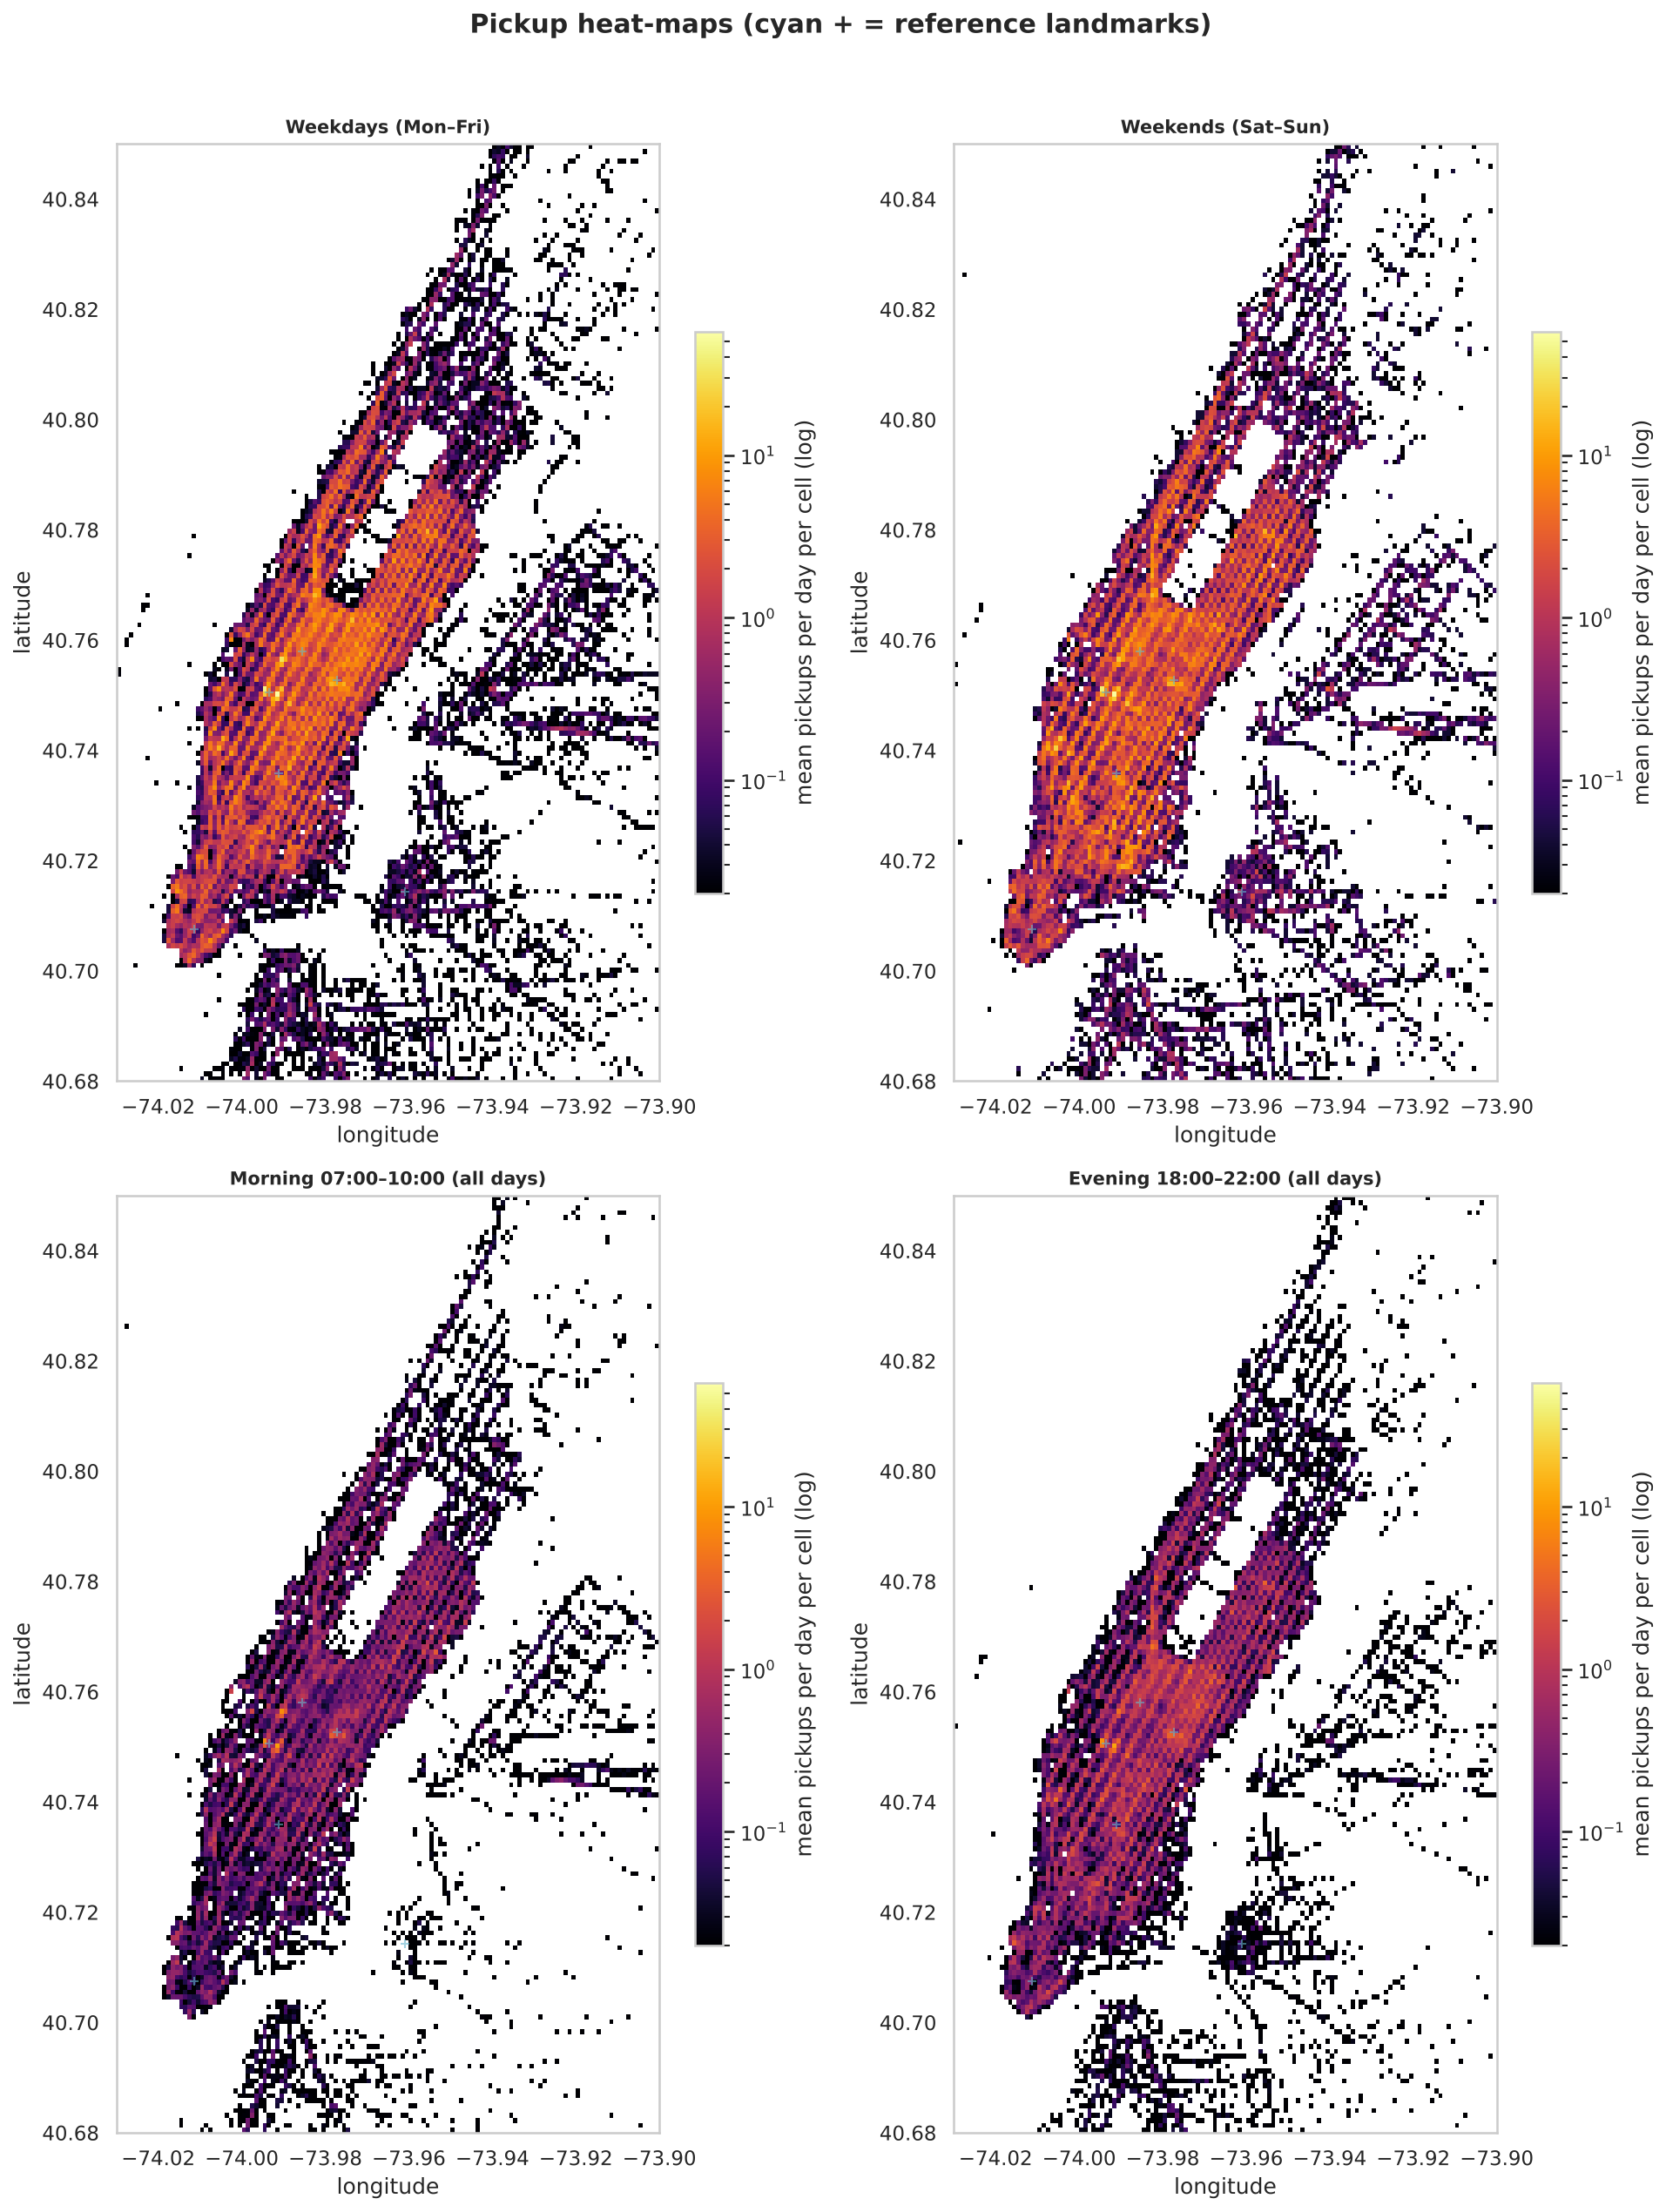
\includegraphics[width=0.72\linewidth]{q4_1_heatmaps_four}\caption{Pickup heat-maps (log density).}\label{fig:heat}\end{figure}
\fig[0.95\linewidth]{q4_1_difference_maps}{Weekend minus weekday and evening minus morning difference in share of pickups (red = relatively more of the first group).\label{fig:diff}}
\textbf{Findings.} About 93\,\% of pickups are in Manhattan; the avenue grid is clearly visible, while the other boroughs are sparse and the airports (JFK and LaGuardia, about 2\,\% each) are isolated spots. Newark has essentially none. \emph{Weekdays vs weekends:} weekday pickups concentrate in Midtown and on the East Side (Midtown within 2\,km of Times Square holds 45.0\,\% of weekday pickups vs 39.9\,\% at weekends; Grand Central 8.9\,\% vs 6.4\,\%; Upper East Side 21.8\,\% vs 18.1\,\%), whereas at weekends activity shifts downtown to nightlife districts (East Village/Lower East Side 6.8\,\% $\to$ 10.9\,\%; the difference map is red over the Lower East Side, East/West Village and Chelsea). \emph{Morning vs evening:} mornings come from residential areas (Upper East Side 26.1\,\% of morning vs 19.5\,\% of evening pickups; Penn Station 8.3\,\% vs 7.1\,\%), evenings from Midtown (46.4\,\% vs 42.1\,\%) and the downtown dining and nightlife areas (7.2\,\% vs 6.0\,\%). The spatial pattern therefore mirrors Section~3: a residential-to-business flow in the morning, the reverse in the evening, and a leisure geography at weekends.

\subsection{Hotspots}
We study Friday 23:00 -- Saturday 02:00 and Thursday 17:00 -- 20:00, pooled over the 26 weeks (storm excluded): 33\,712 and 37\,805 pickups in 76 and 78 separate clock-hours, i.e.\ only 444--485 pickups per hour for the whole city.

\textbf{The suggested definition cannot be met.} A hotspot of ``at least 15 pickups within 50 or 100 m in an hour'' never occurs: in every single hour of both windows the largest number of pickups within 100 m of one another is 14 (10--11 within 50 m), so the literal rule finds zero hotspots. The training file is a sample of taxi activity and absolute thresholds from the brief are too high. We keep the idea (a persistent \emph{rate} of pickups) and set \texttt{min\_samples} $=$ (required pickups per hour) $\times$ (number of pooled clock-hours), with haversine DBSCAN (ball tree).

\textbf{Parameters.} $\varepsilon=50$\,m: a NYC block is about 80\,m$\times$270\,m and consumer GPS is accurate to 10--50\,m, so 50\,m is about one street corner and gives drivers a place they can drive to. With $\varepsilon=100$\,m DBSCAN \emph{chains} neighbouring blocks (the largest cluster has radius 1.2--1.5\,km at 1 pickup/hour, i.e.\ most of Midtown becomes one blob). A rate of \textbf{1 pickup per hour} (\texttt{min\_samples} $=76$ and $78$) gives compact clusters (largest radius $<200$\,m); 0.5/hour gives over 100 clusters that begin to chain, 2/hour leaves only 6 (Table~\ref{tab:grid}).
\begin{table}[!htbp]\centering\small
\caption{Number of clusters (largest cluster radius in metres) for different $\varepsilon$ and required pickups per hour; Friday night | Thursday evening.}\label{tab:grid}
\begin{tabular}{lcccccc}\toprule & \multicolumn{3}{c}{Fri 23:00--02:00} & \multicolumn{3}{c}{Thu 17:00--20:00}\\ $\varepsilon$ (m) & 0.5/h & 1/h & 2/h & 0.5/h & 1/h & 2/h\\\midrule
30 & 77 (183) & 12 (60) & 0 & 47 (119) & 8 (69) & 3 (54)\\
50 & 116 (484) & \textbf{36 (193)} & 6 (77) & 115 (603) & \textbf{22 (154)} & 6 (139)\\
75 & 90 (1083) & 57 (417) & 15 (196) & 104 (2586) & 43 (743) & 7 (188)\\
100 & 48 (3289) & 47 (1190) & 21 (401) & 60 (4651) & 42 (1502) & 18 (292)\\\bottomrule\end{tabular}
\end{table}
\textbf{Result: 36 hotspot clusters for Friday 23:00--02:00 and 22 for Thursday 17:00--20:00} (Figure~\ref{fig:hot}; interactive folium maps are in \texttt{maps/}). They are compact (radius under 200\,m) and contain 18.5\,\% and 10.4\,\% of the window's pickups; the rest is noise, so demand is mostly diffuse. With $\varepsilon=100$\,m and 2/hour the counts would be 21 and 18, so the number is best read as ``a few dozen''.
\fig[0.95\linewidth]{q4_2_hotspot_maps}{DBSCAN hotspots ($\varepsilon=50$\,m, $\geq1$ pickup/hour); grey = noise, numbers = ten busiest clusters (the airport clusters lie outside this map window).\label{fig:hot}}

\textbf{Where are they?} (Nearest hand-entered landmark; approximate.) \emph{Friday night} is downtown nightlife: 52.6\,\% of the clustered pickups lie in the Village/East Village/Lower East Side/Meatpacking area (vs 3.9\,\% on Thursday), the busiest clusters being around Astor Place/NoHo, Nolita/Bowery on the Lower East Side, the Meatpacking District/West Chelsea (three clusters) and the West Village (2.7--5.2 pickups/hour each), plus Penn Station/Madison Square Garden (3.5/h) and a JFK cluster (2.4/h). \emph{Thursday evening} is transport hubs and the airports: Midtown West (Penn Station, Port Authority, Columbus Circle, Fifth Avenue/57th) holds 40.7\,\% of clustered pickups (15.9\,\% on Friday), the Upper East/West Side 21.1\,\% (0\,\% on Friday), and the busiest cluster is the LaGuardia terminal area (6.9/h) followed by two Penn Station clusters (5.3 and 3.9/h). Only 7 of the 36 Friday clusters have a Thursday cluster within 250\,m. A driver should therefore wait at the airports and Penn Station/Port Authority/Columbus Circle on Thursday early evening, and in the East Village--Lower East Side--Meatpacking--West Village area after 23:00 on Friday. Limitations: pooling averages out weather and events; a single $\varepsilon$ cannot suit both dense Midtown and sparse areas (80--90\,\% of pickups are noise); airports are hotspots in one direction only.

%====================================================================
\section{Airports}
A trip is an Empire State Building (ESB) $\to$ airport trip if its pickup lies within $R_\text{ESB}$ of the ESB and its dropoff within $R_\text{air}$ of the airport centre (haversine; cleaned data; time of day = pickup hour). The brief labels the points ``(long, lat)'' but the numbers are (lat, lon) -- 40.65\,N, 73.78\,W is JFK -- and are used so. The straight-line distances are ESB--JFK 21.1\,km, ESB--Newark 17.6\,km.

\textbf{Radii.} Drop-offs around an airport rise steeply with radius to about 1.2\,km (JFK) and 1\,km (Newark) and then flatten, and the drop-off density per km$^2$ falls by one to two orders of magnitude at the same radius (Figure~\ref{fig:rad}); $R_\text{air}=2$\,km contains the terminal area with a margin for GPS error and service roads (only about 600 more JFK drop-offs than 1.2\,km) without including unrelated places. $R_\text{ESB}=0.5$\,km (about two long or six short blocks) covers where passengers actually hail cabs (Herald Square, Penn Station, Fifth Avenue) and gives 862 JFK and 236 Newark trips. The result is robust: the median travel time stays between 45.1 and 47.6 min for JFK and between 32.7 and 35.8 min for Newark for every combination of $R_\text{ESB}\in[0.2,1.0]$\,km and $R_\text{air}\in[1,3]$\,km.
\fig{q5_radius_choice}{Choice of radii: cumulative drop-offs and ring density around the airports, and median travel time versus the ESB radius.\label{fig:rad}}

\begin{table}[!htbp]\centering\small
\caption{Travel time from the Empire State Building (minutes).}\label{tab:air}
\begin{tabular}{lrrrrrrr}\toprule & Trips & Mean & Median & Std & IQR & Distance (km) & Speed (km/h)\\\midrule
JFK & 862 & 49.1 & 46.0 & 17.1 & 36.6--59.9 & 20.9 & 28.6\\ Newark & 236 & 36.3 & 33.1 & 11.8 & 28.3--40.9 & 17.9 & 31.8\\\bottomrule\end{tabular}
\end{table}
\textbf{Results.} Travel to JFK takes on average 49.1 min (median 46.0 min); to Newark 36.3 min (median 33.1 min). JFK is about 13 min (35--40\,\%) slower (Mann--Whitney $p\approx10^{-31}$): it is about 20\,\% further and the trips are slower (28.6 vs 31.8 km/h; plausibly the Queens expressways versus a tunnel and New Jersey highways -- the routes are not in the data). \textbf{By time of day} (Figure~\ref{fig:air}): to JFK the trip takes about 28--33 min between 01:00 and 05:00, 38--41 min at 07:00--10:00, 43--46 min at 11:00--13:00, then jumps to 58 min at 14:00 and peaks at \textbf{66 min at 16:00} (more than twice the night time), falling back to 43 min by 19:00. Period medians for JFK are 28.6 (00--05), 35.4 (06--09), 48.7 (10--15), \textbf{59.6} (16--19) and 39.8 min (20--23). Newark has the same shape at a lower level: 26--29 min at 04:00--06:00, 32--37 min in the morning and midday, 42--45 min at 14:00--16:00 and a peak at 17:00 (59 min, but based on only 4 trips); period medians 27.1, 32.8, 34.0, 42.0 and 32.7 min. The afternoon rush costs 2.1$\times$ the night time to JFK but 1.55$\times$ to Newark. Weekends are faster (JFK median 39.9 vs 50.4 min; Newark 30.6 vs 34.0 min). In practice allow about 45 min to JFK (about an hour in the afternoon rush, 30 min at night) and 33 min to Newark (45 min at 14:00--17:00). Newark has no trips before 04:00 and few after 20:00, and hours with fewer than 5 trips have no confidence interval, so single hours should be read through the confidence bands.
\fig{q5_travel_time_by_hour}{Travel time from the ESB by pickup hour: mean (with 95\,\% bootstrap CI), median, IQR and number of trips.\label{fig:air}}

%====================================================================
\section{Dimensionality reduction}
Everything uses a random sample of 20\,000 cleaned trips (seed 42).

\subsection{Feature matrix}
The 11 features are: pickup and dropoff longitude/latitude; $\log$ distance, $\log$ duration and $\log$ speed (skewness 2.8, 2.15, 1.46 $\to$ 0.37, $-0.13$, $-0.20$, so that a few long airport trips do not dominate Euclidean distances); the cyclic hour encoding $(\sin\frac{2\pi h}{24},\cos\frac{2\pi h}{24})$ so that 23:00 and 00:00 are neighbours; and the same cyclic encoding of the day of week with period 7. All features are standardised (\texttt{StandardScaler}), which is essential because PCA, t-SNE, UMAP and DBSCAN are distance/variance based: without it duration in seconds would swamp coordinates in degrees and the unit-circle encodings. A consequence worth stating in advance: day of week takes only seven values, so every trip sits on one of seven fixed points in two of the 11 coordinates, which leaves a strong imprint on the embeddings. The 11th principal component has zero variance because $\log\text{speed}=\log\text{distance}-\log\text{duration}+\text{const}$.

\subsection{PCA}
The variance is spread out: PC1 explains 22.1\,\%, PC2 13.9\,\%, PC3 12.3\,\%, PC4 10.2\,\%, so two components capture only 36.0\,\% and \textbf{8 components are needed for 90\,\%} (83.7\,\% with 7, 90.2\,\% with 8; Figure~\ref{fig:scree}). Loadings (Figure~\ref{fig:load}): \textbf{PC1} (22\,\%) is trip length and speed (distance $+0.60$, duration $+0.46$, speed $+0.36$, pickup longitude $+0.35$): long, fast trips towards Queens/the airports; \textbf{PC2} (14\,\%) is the uptown--downtown (north-east) position (dropoff latitude $+0.61$, pickup latitude $+0.53$); \textbf{PC3} (12\,\%) is time of day (hour\_cos $+0.61$, speed $+0.48$, duration $-0.44$: fast short night trips versus slow afternoon trips); \textbf{PC4} is almost purely hour\_sin ($+0.78$), the morning--evening contrast. On the first two components (Figure~\ref{fig:pca}) distance is the only clearly structured colouring: long trips form separate small clouds at PC1 $\approx$ 2.5--3 and 5--6 (the airport groups), whereas hour and weekday/weekend overlap completely because they load on later components. A two-component PCA therefore separates long from short trips and uptown from downtown, but not \emph{when}.
\begin{figure}[!htbp]\centering
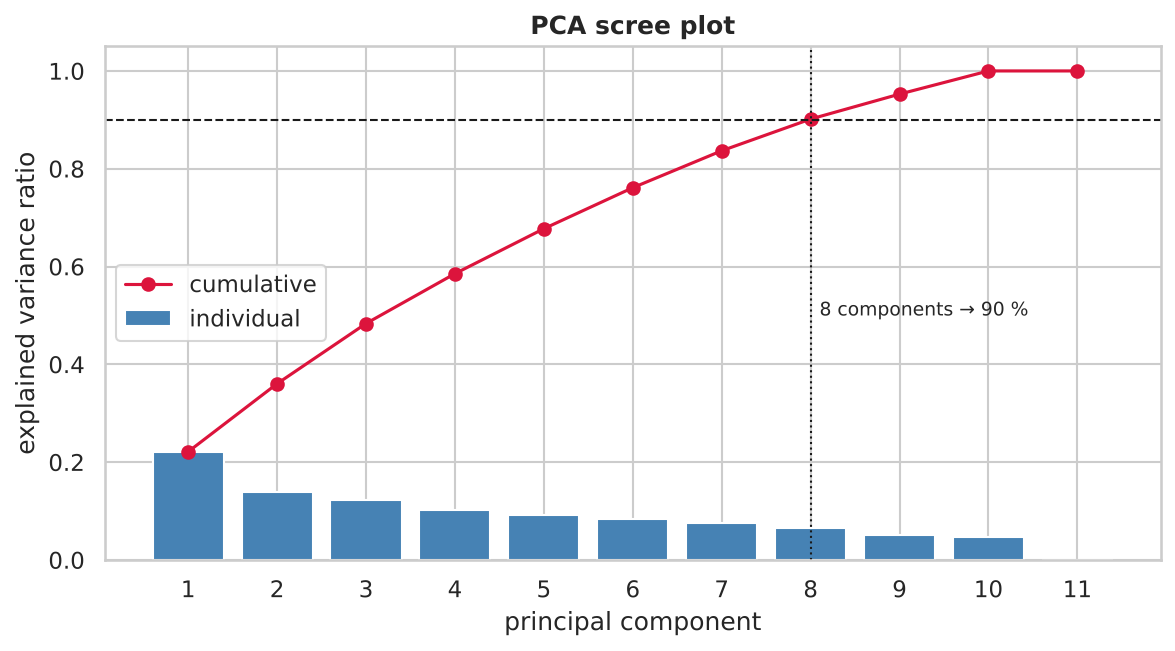
\includegraphics[width=0.48\linewidth]{q6_2_scree}\hfill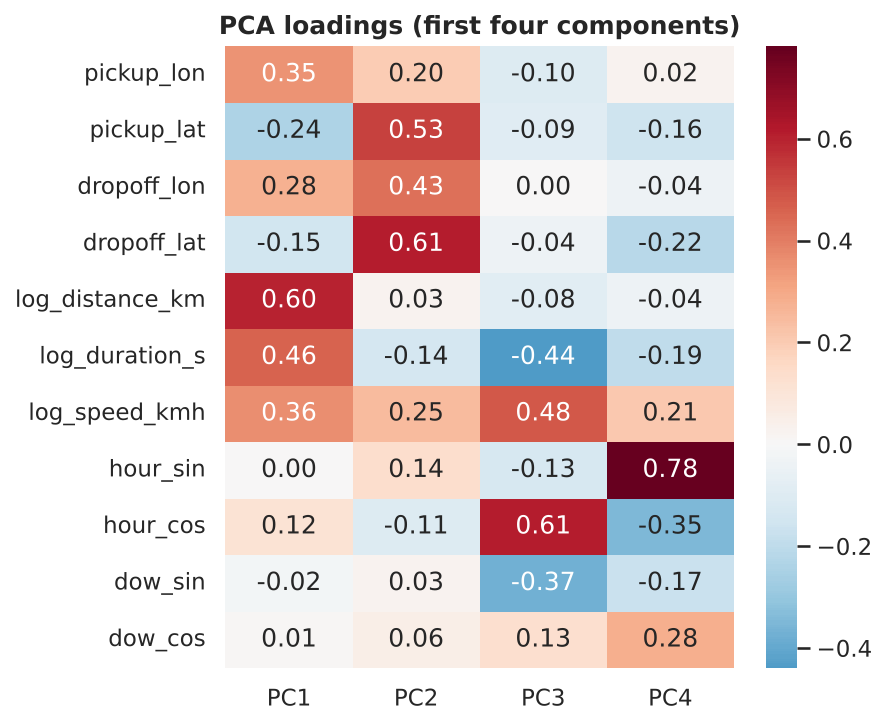
\includegraphics[width=0.40\linewidth]{q6_2_loadings}
\caption{PCA scree plot with cumulative explained variance (left) and loadings of the first four components (right).}\label{fig:scree}\label{fig:load}
\end{figure}
\fig{q6_2_pca_scatter}{PCA, first two components, coloured by pickup hour, weekday/weekend and trip distance.\label{fig:pca}}

\subsection{t-SNE}
Figure~\ref{fig:tsne} shows t-SNE (PCA initialisation, seed 42) with perplexity 5, 30 and 100. \textbf{Perplexity 5} (57 s) is very local: one nearly circular blob without clear groups, with fragmented chains of long trips; it over-emphasises noise. \textbf{Perplexity 30} (69 s) shows a flower of about seven large lobes and several small separate islands: colouring by weekend shows that the lobes are the days of the week (two weekend lobes) with the hour changing smoothly inside each, and the islands on the right are the long (airport) trips. \textbf{Perplexity 100} (110 s) shows the same groups as fewer, larger, more compact lobes with better separation and cleaner hour gradients, but small structures begin to be absorbed, the cost grows and the relative positions of the lobes change -- the distances between islands are not stable, only their membership.

\textbf{Reproducibility note.} t-SNE is not exactly repeatable here: even with a fixed seed, a clean re-run of the whole notebook (new environment, no cached results) gave 24 instead of 19 DBSCAN clusters on the chosen t-SNE embedding (2.9\,\% instead of 2.6\,\% noise) and a t-SNE--UMAP ARI of 0.45/0.48 instead of 0.42/0.45 (Section~6.6), probably because of floating-point differences in the multi-threaded implementation; the UMAP clustering was identical (29 clusters, 3.5\,\% noise). The numbers quoted in this report are those of the run saved in the notebook; the conclusions do not depend on the exact values.
\begin{figure}[!htbp]\centering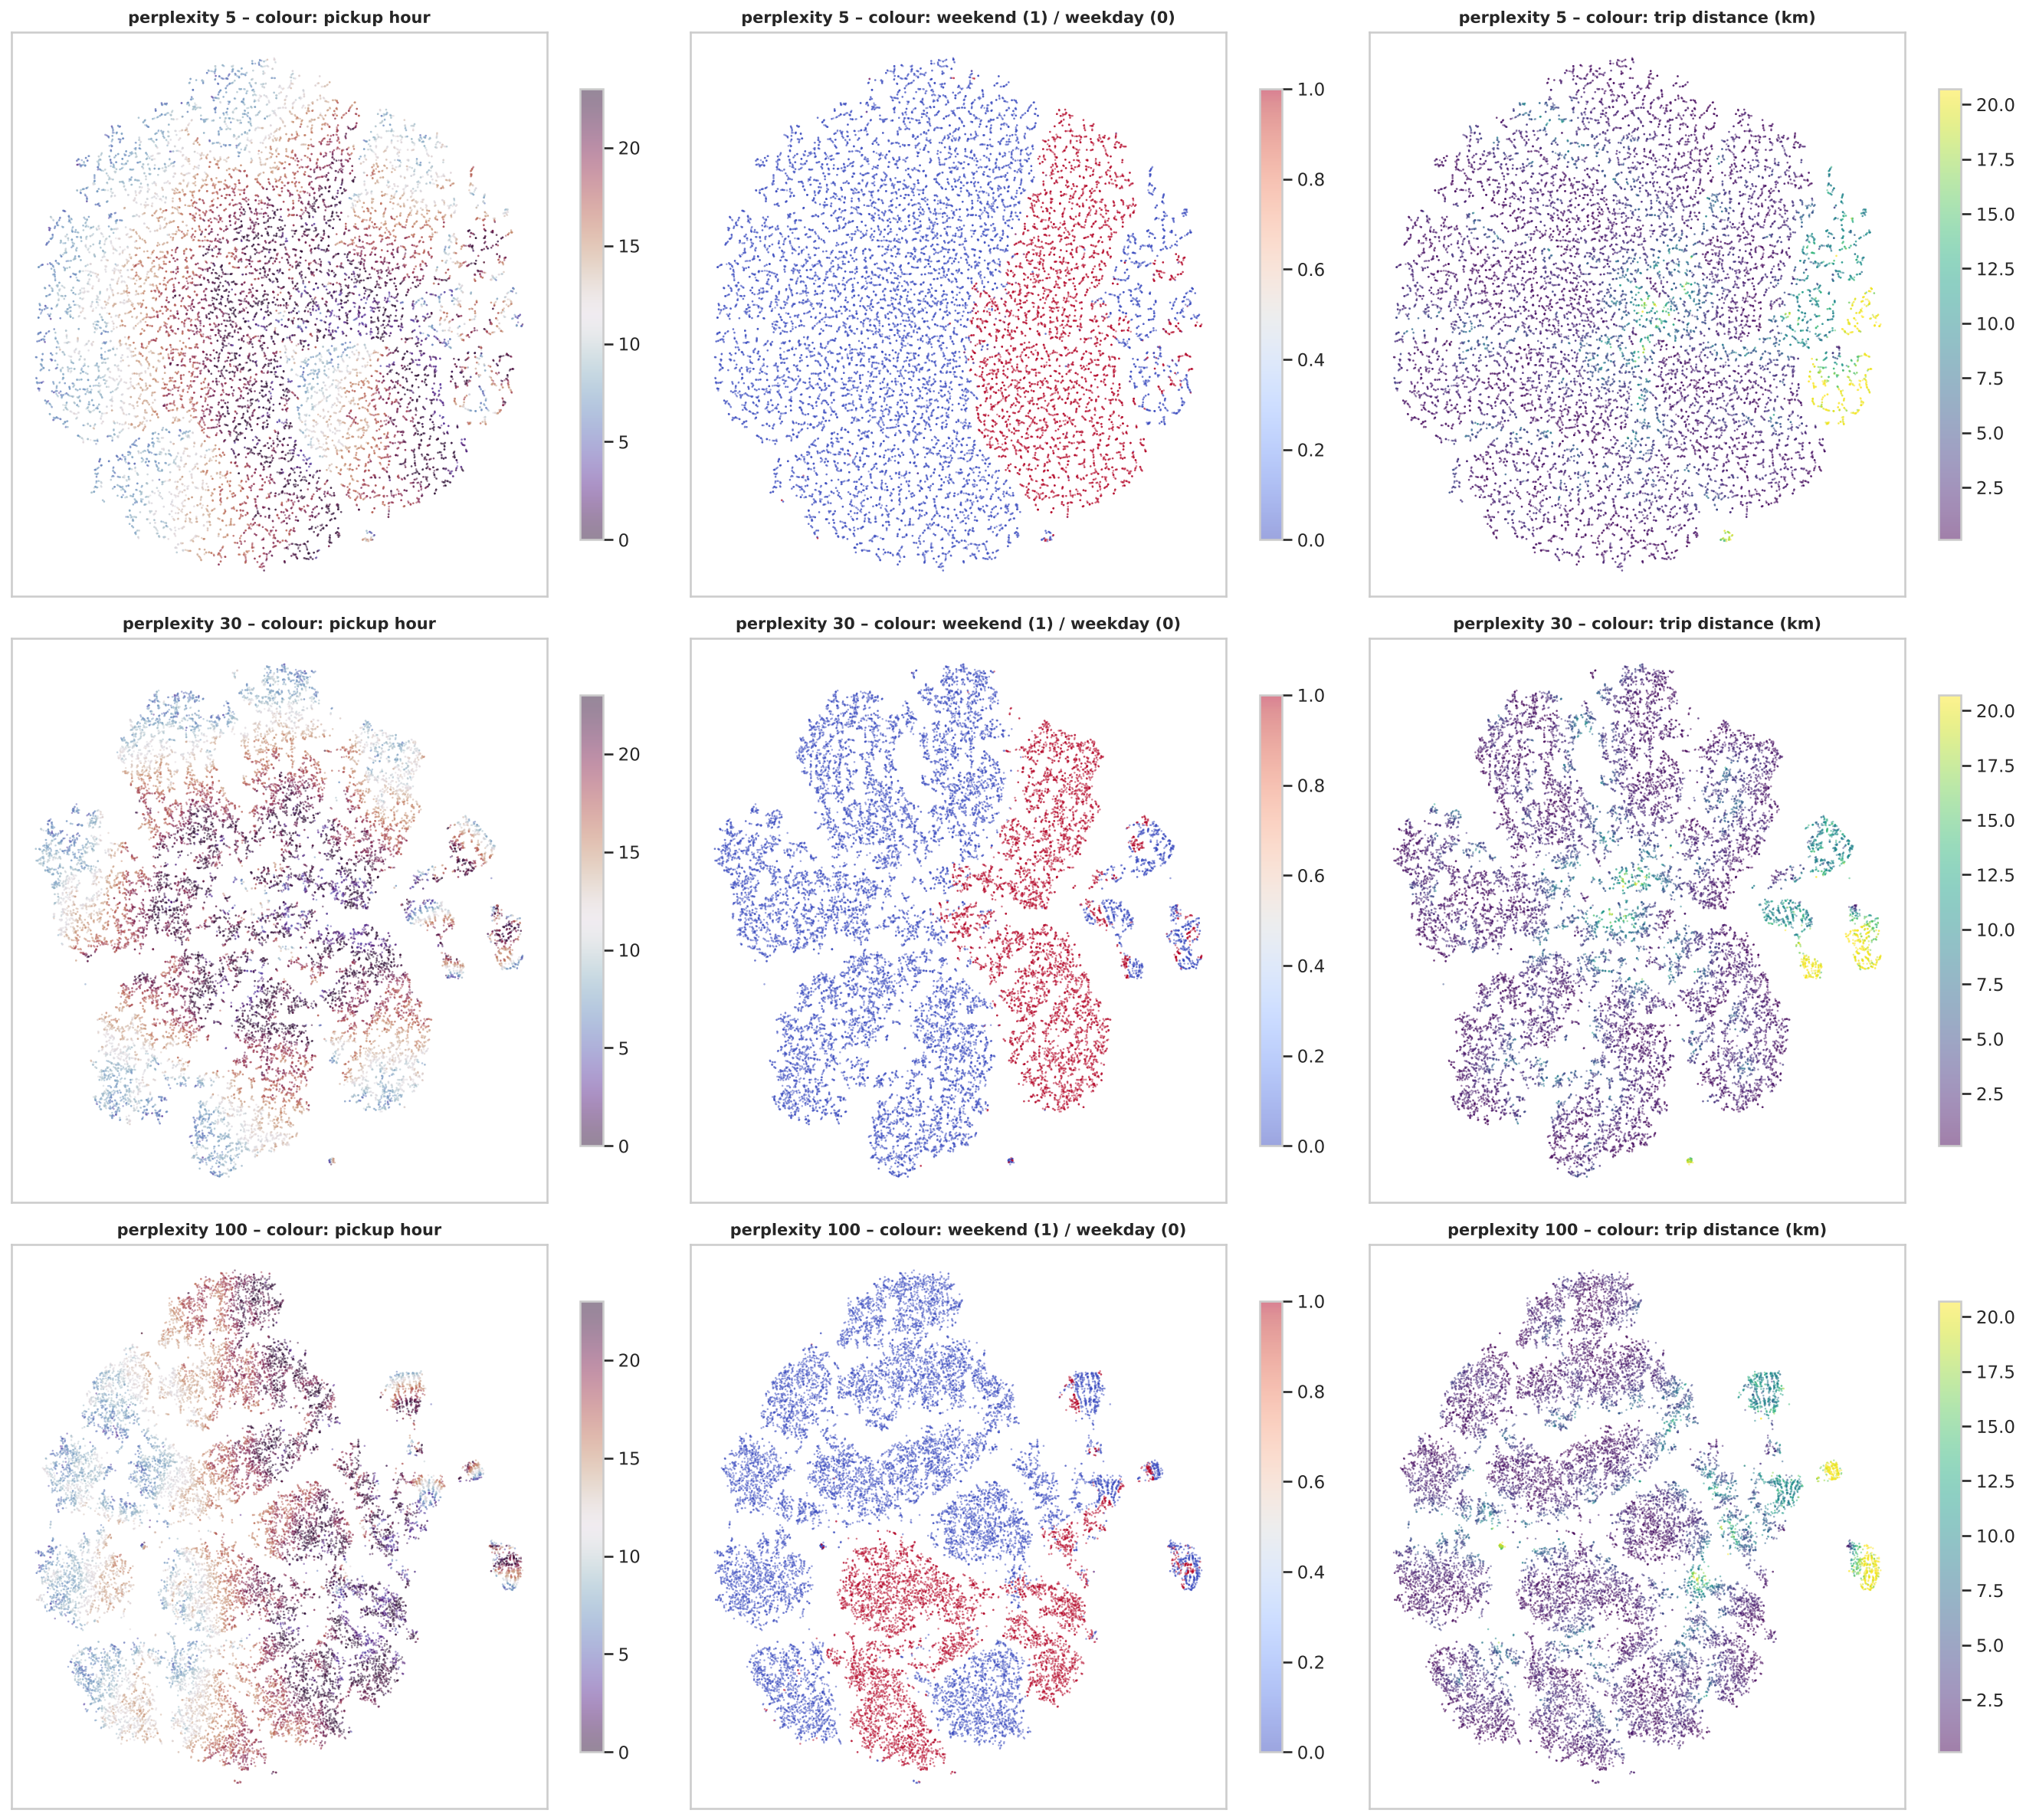
\includegraphics[width=0.93\linewidth]{q6_3_tsne_grid}\caption{t-SNE with perplexity 5 (top), 30 (middle) and 100 (bottom), coloured by pickup hour, weekday/weekend and trip distance.}\label{fig:tsne}\end{figure}

\subsection{UMAP}
UMAP was run for $n_\text{neighbors}\in\{5,15,50\}$ and $\text{min\_dist}\in\{0,0.5\}$ (Figure~\ref{fig:umap}; the weekend and distance colourings are in the notebook). With \textbf{$n_\text{neighbors}=5$} the groups are fragmented with many small satellite pieces (over-segmentation of noise); with \textbf{15} the groups are compact and complete and the airport islands are visible; with \textbf{50} the daily groups are most regular, a flower of seven petals, and fine detail is smoothed away: larger $n_\text{neighbors}$ trades local detail for a cleaner, more global arrangement. \textbf{$\text{min\_dist}=0$} packs points into tight, clearly separated islands with white space between them (ideal for clustering, but it hides density differences inside a group and exaggerates gaps); \textbf{$0.5$} spreads points so that the internal hour gradient is visible but groups touch and boundaries blur. In all six settings the message is the same: seven day-of-week groups (two weekend) with smooth hour gradients, and a handful of small groups of long trips. UMAP took 6--30 s per setting (the first includes numba compilation) against 57--110 s for t-SNE.
\begin{figure}[!htbp]\centering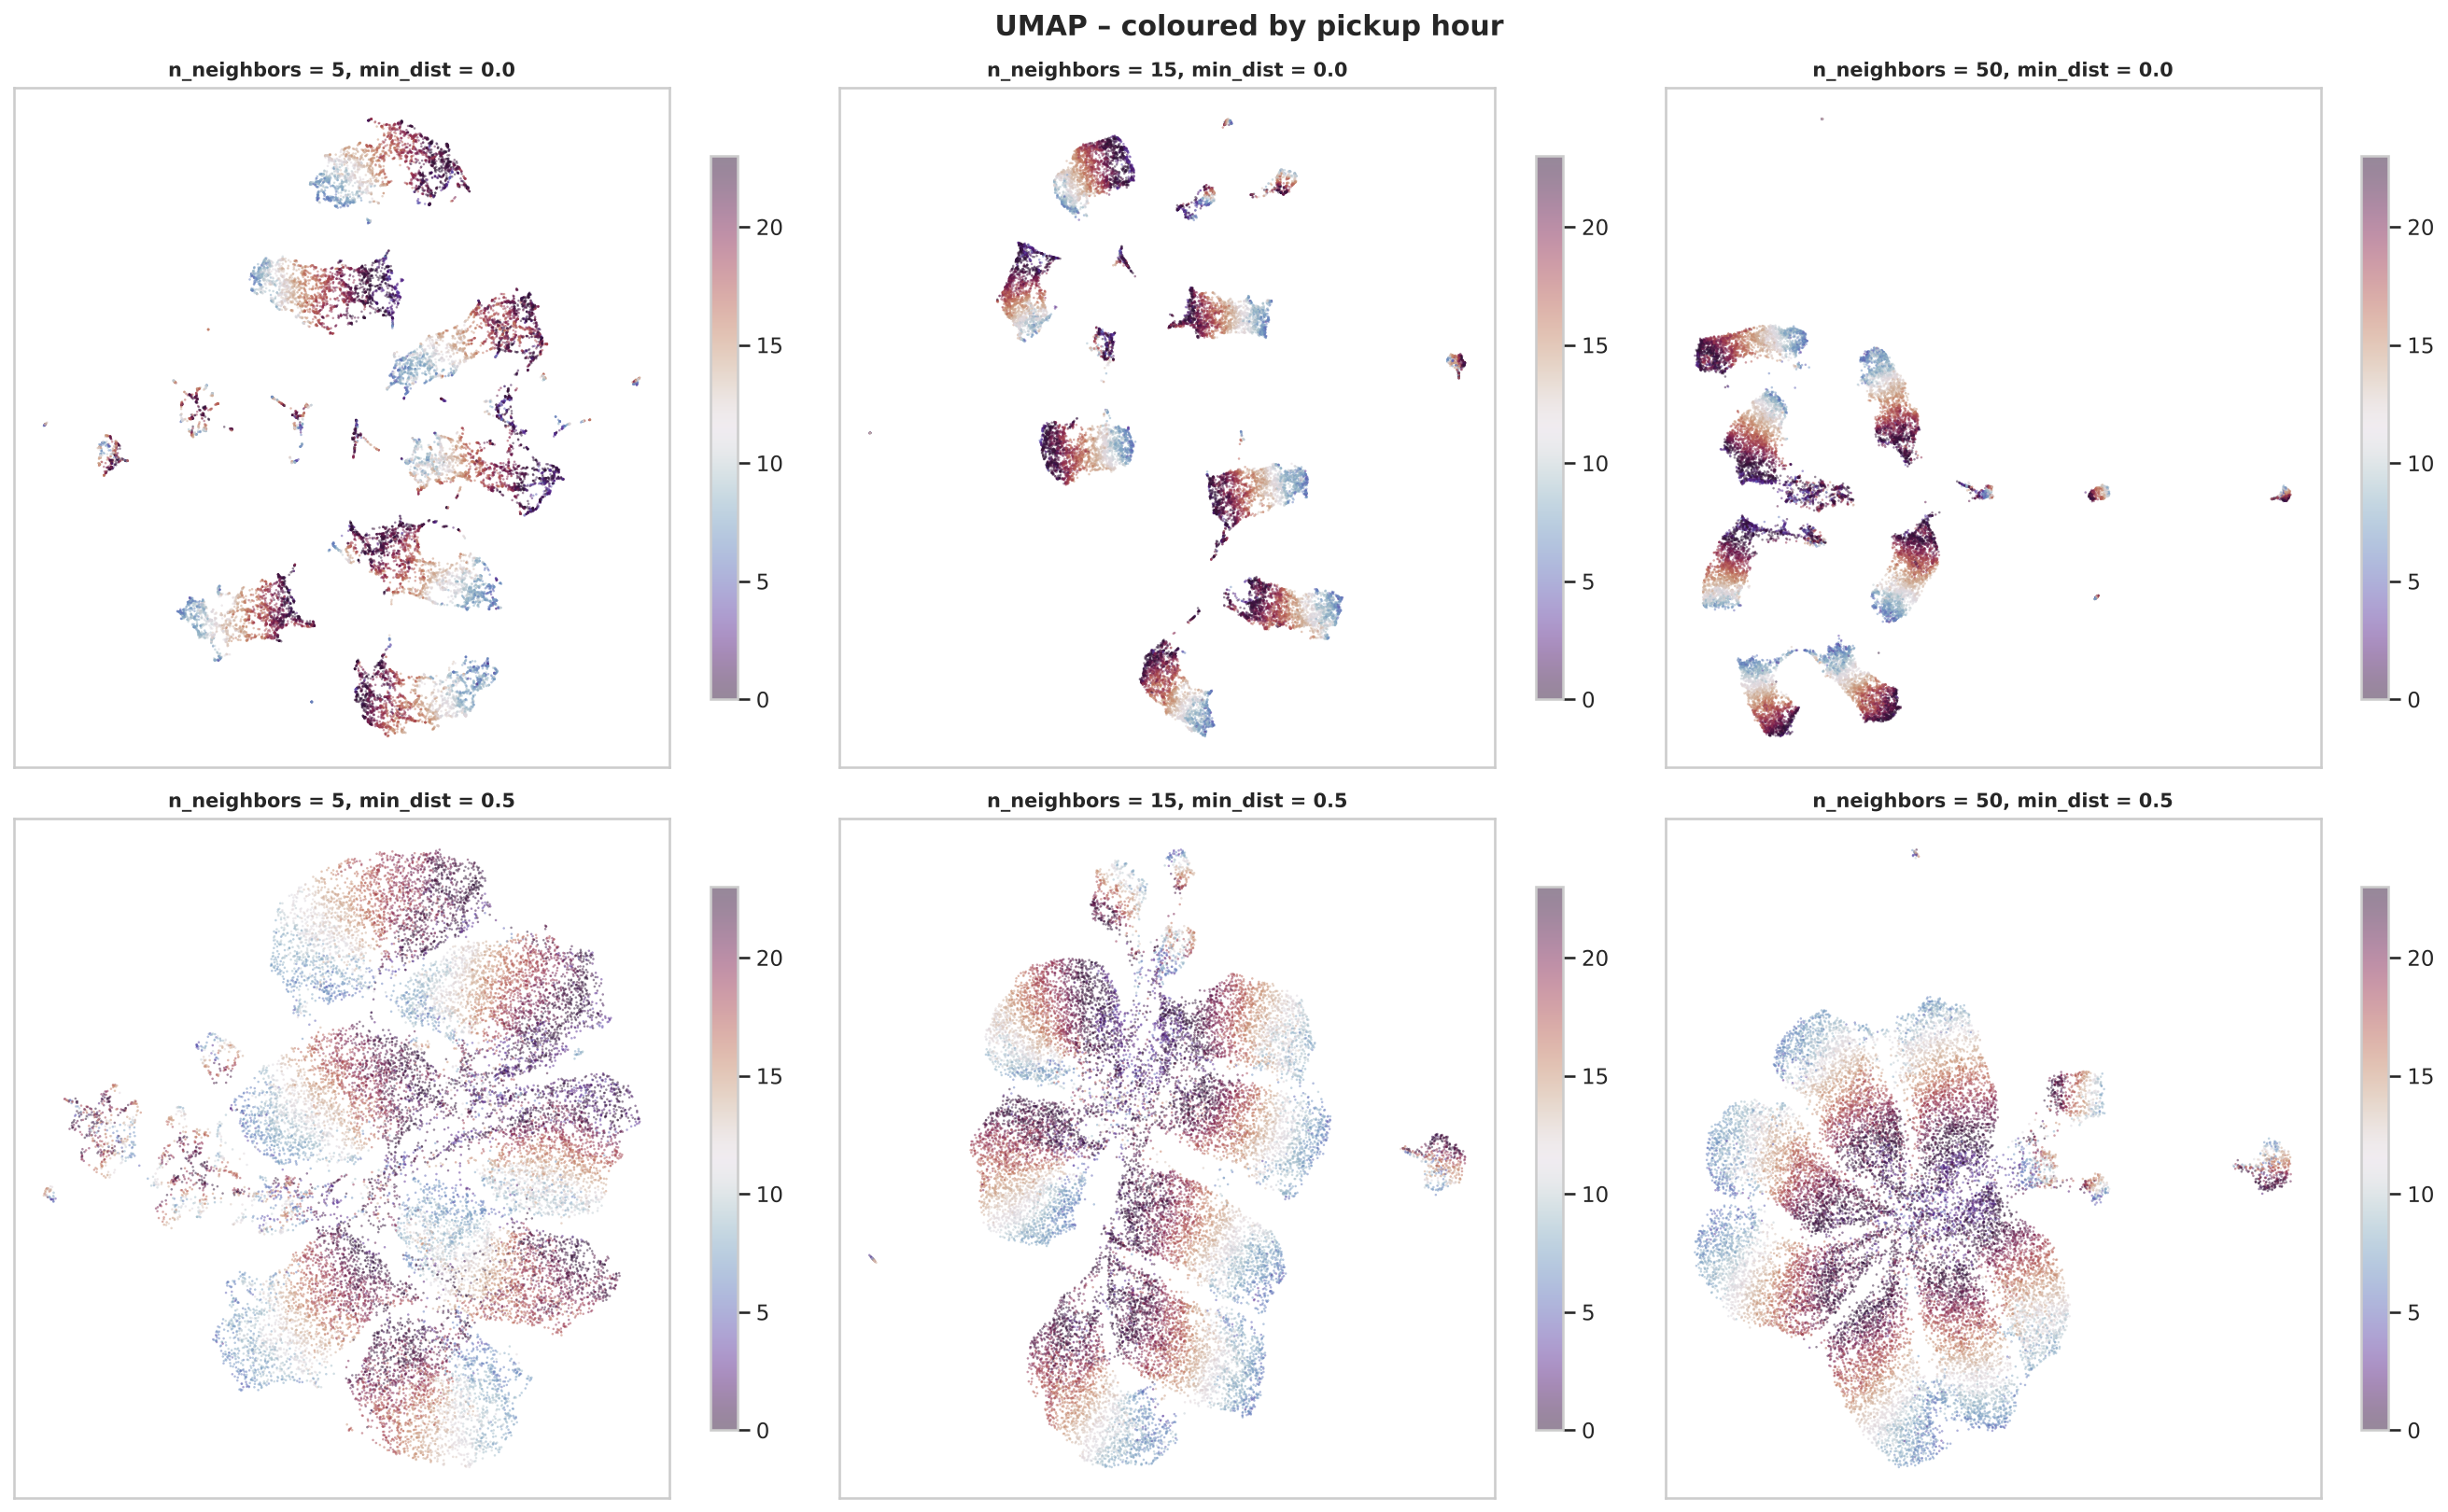
\includegraphics[width=0.93\linewidth]{q6_4_umap_hour}\caption{UMAP embeddings coloured by pickup hour: columns $n_\text{neighbors}=5,15,50$, rows $\text{min\_dist}=0,0.5$.}\label{fig:umap}\end{figure}

\subsection{Density-based clustering and cluster profiles}
\textbf{Best embedding.} We choose the best t-SNE/UMAP embedding quantitatively with the \emph{trustworthiness} (fraction of each point's 15 nearest embedded neighbours that are also near neighbours in the original space; 4\,000-trip subset) and the Spearman correlation of pairwise distances (global structure) (Table~\ref{tab:trust}): t-SNE perplexity 100 (0.980, just ahead of perplexity 30 with 0.977) and UMAP $n_\text{neighbors}=50$, $\text{min\_dist}=0$ (0.960) are selected.
\begin{table}[!htbp]\centering\small
\caption{Quality of the 2-D embeddings.}\label{tab:trust}
\begin{tabular}{lrr}\toprule Embedding & Trustworthiness ($k=15$) & Distance correlation\\\midrule
PCA, 2 components & 0.768 & 0.750\\ t-SNE perplexity 5 / 30 / 100 & 0.945 / 0.977 / \textbf{0.980} & 0.323 / 0.329 / 0.405\\
UMAP $n=5$, md 0 / 0.5 & 0.956 / 0.918 & 0.223 / 0.220\\ UMAP $n=15$, md 0 / 0.5 & 0.954 / 0.929 & 0.286 / 0.304\\ UMAP $n=50$, md 0 / 0.5 & \textbf{0.960} / 0.929 & 0.363 / 0.386\\\bottomrule\end{tabular}
\end{table}
\textbf{Method and parameters.} DBSCAN with \texttt{min\_samples}$=30$ for all methods (a cluster must contain at least 30 trips, 0.15\,\% of the sample) and $\varepsilon$ from the knee of the sorted 30-th-neighbour distance plot (Figure~\ref{fig:kd}): $\varepsilon=1.42$ (PCA), 2.53 (t-SNE), 0.16 (UMAP); they differ because the spaces have different scales. PCA is clustered in the 8 dimensions that explain 90\,\% of the variance and visualised on the first two components; t-SNE and UMAP are clustered on the 2-D embeddings.
\fig{q6_5_kdistance}{k-distance plots (k=30) with the chosen $\varepsilon$ (dashed).\label{fig:kd}}
\fig{q6_5_clusters_2d}{DBSCAN clusters (noise grey) in the three spaces.\label{fig:cl}}
\begin{table}[!htbp]\centering\small
\caption{Clustering results.}\label{tab:cl}
\begin{tabular}{lrrrr}\toprule Method (space) & $\varepsilon$ & Clusters & Noise & Largest cluster\\\midrule
PCA (8 PCs) & 1.42 & 6 & 8.9\,\% & 88.7\,\%\\ t-SNE (perplexity 100) & 2.53 & 19 & 2.6\,\% & 29.1\,\%\\ UMAP (50 neighbours, min\_dist 0) & 0.16 & 29 & 3.5\,\% & 12.9\,\%\\\bottomrule\end{tabular}
\end{table}
\textbf{PCA} finds one giant cluster (88.7\,\%: median 1.95 km, 10.3 min, 12.2 km/h, spread over the day and week) plus a few small airport clusters (23--246 trips); its noise group is half airport trips (median distance 10.5 km). So PCA with density clustering separates only ``airport/long'' from ``everything else''. \textbf{t-SNE} (19 clusters) isolates Thursday midday and evening, Friday midday, Tuesday and Wednesday mornings and Sunday late night, but merges Saturday and Sunday (and some weekday trips) into one cluster (29.1\,\%) and several weekdays into another (26.4\,\%); six small clusters are airport runs. \textbf{UMAP} (29 clusters) finds each day of the week as its own cluster (Monday, Tuesday, Wednesday, Friday, Saturday, Sunday each 8--13\,\% of the sample and 99--100\,\% one day; Thursday split into a midday and an evening cluster; Sunday also has a small late-night cluster, i.e.\ Saturday night after midnight) plus small clusters of long trips. Table~\ref{tab:prof} profiles the main UMAP clusters on the original (unscaled) features; the names come from a fixed rule applied to these statistics (time of day from the circular mean hour; weekday/dominant day; length from the median distance; ``airport runs'' if more than 50\,\% of the trips start or end within 2\,km of JFK, LaGuardia or Newark), so they are reproducible and consistent with the numbers.
\begin{table}[!htbp]\centering\scriptsize
\caption{Profile of selected UMAP clusters (original features; hour = circular mean; ``airport'' = share of trips within 2\,km of JFK/LGA/Newark).}\label{tab:prof}
\begin{tabular}{llrrrrrrr}\toprule Name & Cl. & \% & Dist (km) & Dur (min) & Speed & Hour & Weekend & Airport\\\midrule
all-day Fri short trips & 8 & 12.9 & 1.79 & 10.0 & 11.1 & 16.6 & 0.00 & 0.00\\
all-day Sat short trips & 3 & 12.8 & 1.90 & 9.4 & 12.7 & 17.5 & 1.00 & 0.00\\
all-day Wed short trips & 2 & 12.1 & 1.77 & 10.4 & 10.7 & 16.2 & 0.00 & 0.00\\
all-day Tue short trips & 4 & 11.8 & 1.75 & 9.7 & 11.3 & 15.8 & 0.00 & 0.00\\
all-day Mon short trips & 10 & 10.2 & 1.73 & 9.1 & 12.1 & 15.8 & 0.00 & 0.00\\
midday Sun short trips & 11 & 8.4 & 1.94 & 8.7 & 13.8 & 14.8 & 1.00 & 0.00\\
midday Thu short trips & 6 & 6.3 & 1.78 & 10.9 & 10.1 & 10.3 & 0.00 & 0.00\\
evening Thu short trips & 5 & 6.1 & 1.97 & 10.1 & 12.1 & 20.2 & 0.00 & 0.00\\
late-night Sun short trips & 13 & 1.9 & 1.81 & 8.1 & 13.7 & 1.4 & 0.99 & 0.00\\
late-night mixed-week long trips & 0 & 1.3 & 9.74 & 19.9 & 29.3 & 23.4 & 0.37 & 0.01\\
midday mixed-week long airport runs (LGA) & 1 & 2.3 & 9.76 & 28.5 & 20.6 & 16.0 & 0.20 & 0.98\\
all-day mixed-week very long airport runs (JFK) & 7 & 2.1 & 19.83 & 40.2 & 27.2 & 17.8 & 0.25 & 0.97\\
midday mixed-week very long airport runs & 12 & 0.8 & 20.47 & 42.8 & 28.7 & 13.2 & 0.37 & 0.88\\\bottomrule\end{tabular}
\end{table}
\textbf{Interpretation.} The great majority are short (1.7--2.0 km, 9--11 min, 10--14 km/h) Midtown/Grand Central/Times Square hops spread over the day, one cluster per day of the week; their speeds reflect the congestion of Section~3.5 (among the all-day clusters Wednesday is slowest at 10.7 km/h and Saturday fastest at 12.7). Thursday splits into the slowest cluster (midday, 10.1 km/h) and an evening cluster. Late-night Sunday (i.e.\ Saturday night) trips are short (1.8 km, 8 min; mean hour 1.4); a fast, long late-night group (9.7 km at 29.3 km/h) probably consists of highway or cross-town night rides. The airport runs form distinct clusters: LaGuardia-area trips (about 9.8 km, 28.5 min) and JFK trips (about 20 km, 40--43 min, 27--29 km/h; two clusters that are probably the two directions of the same route, one centred at JFK and one in Midtown). The pickup maps (Figure~\ref{fig:maps} for UMAP; Figures~\ref{fig:mapspca} and~\ref{fig:mapstsne} in the appendix for PCA and t-SNE) show that the day-of-week clusters cover the same Manhattan footprint, so location does not separate them; only the airport clusters with pickups at an airport are spatially distinct (the others have their pickups in Manhattan, because they are trips towards the airport).
\begin{figure}[!htbp]\centering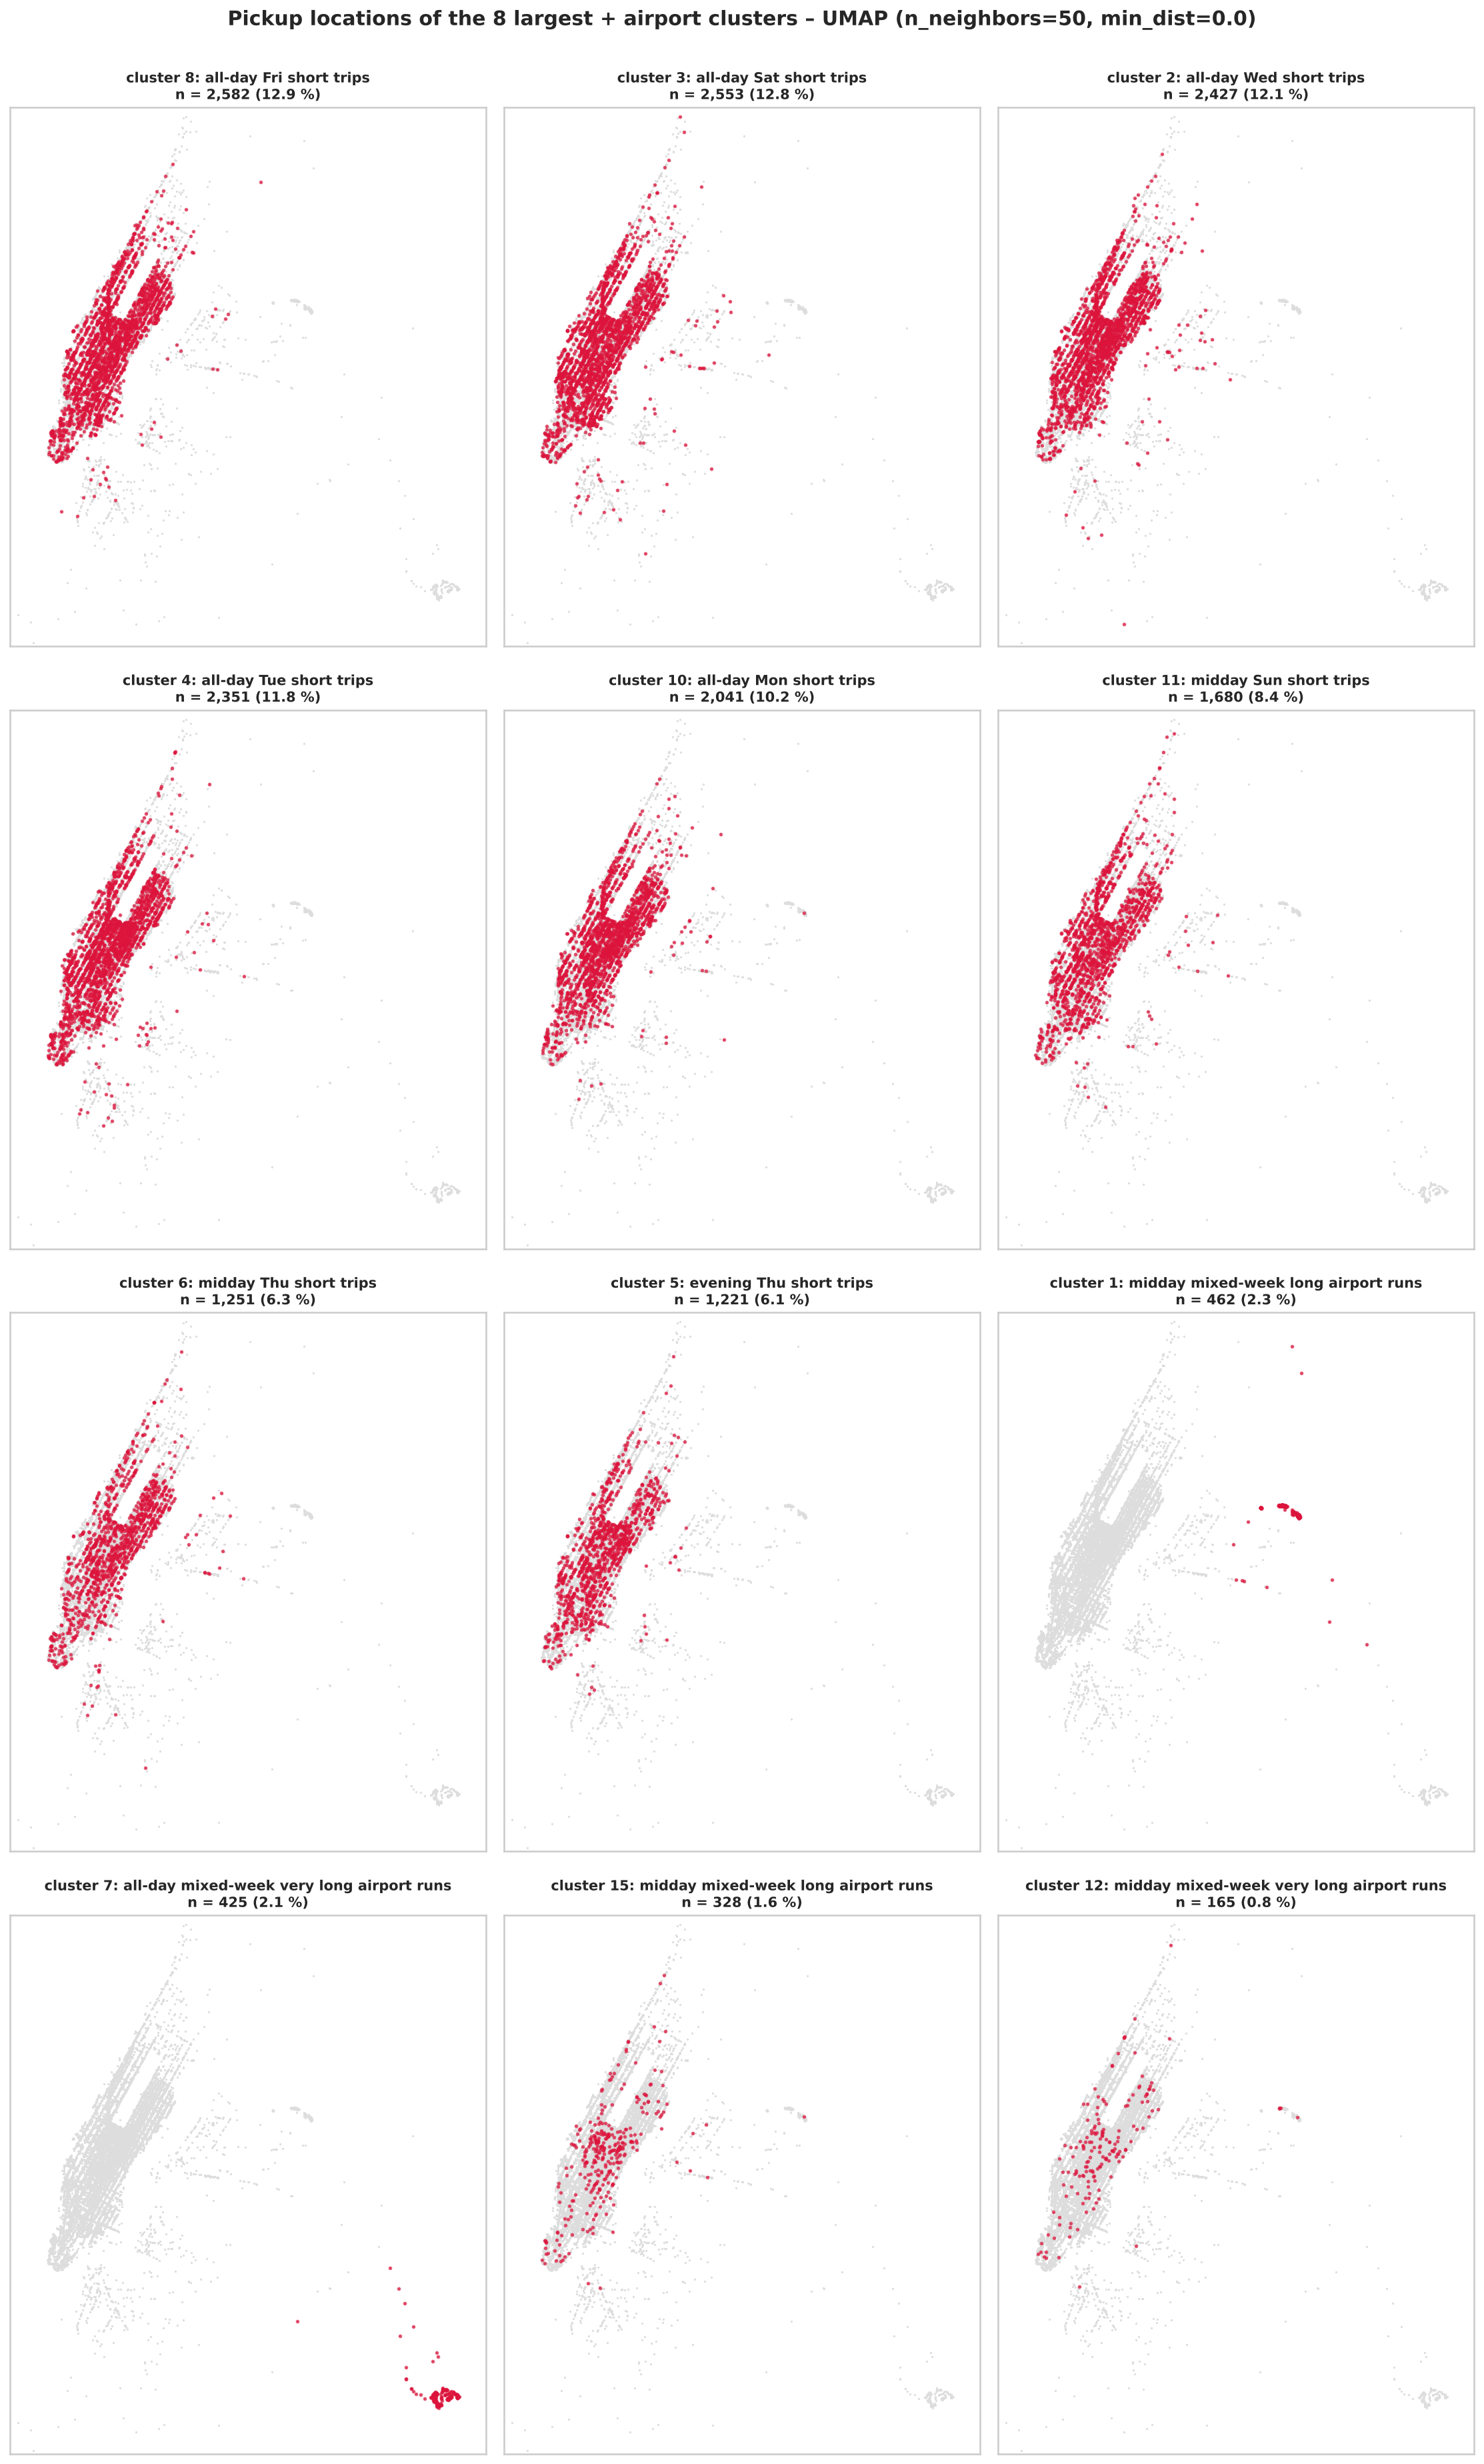
\includegraphics[width=0.74\linewidth]{q6_5_maps_umap}\caption{Pickup locations (red) of the eight largest and the airport-dominated UMAP clusters; grey = all sampled pickups.}\label{fig:maps}\end{figure}

\subsection{Comparison of PCA, t-SNE and UMAP}
\fig{q6_6_side_by_side}{Best embedding of each method side by side; top: coloured by pickup hour; bottom: airport trips (pickup or dropoff within 2\,km of JFK, LaGuardia or Newark; 6.7\,\% of the sample) in red.\label{fig:sbs}}
\textbf{Consistent groups.} \emph{Airport trips form their own group in all three methods}: in t-SNE and UMAP they are compact islands separated from the bulk (UMAP: three well separated islands plus smaller ones), in PCA they lie away from the bulk along the long-trip direction but as a diffuse band overlapping its edge. The seven day-of-week groups and the late-night weekend groups appear in t-SNE and UMAP but not in PCA. \textbf{PCA} reveals the dominant linear axes (interpretable through the loadings), preserves global distances best (distance correlation 0.75 vs 0.41 for t-SNE and 0.36 for UMAP) and takes well under a second, but it misses local structure (trustworthiness 0.77 against 0.98 and 0.96) and cannot resolve the day/time groups or the small airport groups.

\textbf{Local versus global structure.} t-SNE and UMAP preserve neighbourhoods far better than PCA (trustworthiness 0.98/0.96 vs 0.77; UMAP is better with $\text{min\_dist}=0$) but preserve global distances poorly (0.2--0.4 vs 0.75). \emph{Distances between clusters should not be interpreted}: the arrangement of the lobes changes with the perplexity and with the seed (Figure~\ref{fig:seed}), and the gaps are largely created by the algorithm (the silhouette of the clusters in the original space is about zero, below). \emph{Cluster sizes are not interpretable either}: t-SNE equalises point density and UMAP with $\text{min\_dist}=0$ packs points tightly, so the area of an island does not measure its population or spread. Only membership, and to a lesser degree local neighbourhoods, can be read.

\begin{table}[!htbp]\centering\small
\caption{Runtime and sensitivity (20\,000 trips, 4 cores).}\label{tab:rt}
\newcolumntype{L}[1]{>{\raggedright\arraybackslash}p{#1}}
\begin{tabular}{L{1.1cm}L{3.2cm}L{4.0cm}L{4.6cm}}\toprule & Runtime & Hyper-parameters & Seed\\\midrule
PCA & well under 1 s & only number of components & deterministic\\
t-SNE & 57 / 69 / 110 s (perplexity 5 / 30 / 100); 93--116 s with random initialisation & high: perplexity 5 gives no groups; 30 and 100 similar but lobes arranged differently & random initialisation: 21--24 clusters, ARI 0.85 / 0.45 / 0.39 between seeds; with PCA initialisation nearly seed-independent (ARI 1.0, trivially)\\
UMAP & 6--44 s (the first call includes compilation) & high: fragmentation and gap size change with $n_\text{neighbors}$, min\_dist & 29 / 20 / 23 clusters; ARI 0.86, 0.86, 0.90\\\bottomrule\end{tabular}
\end{table}
\fig{q6_6_seed_sensitivity}{Seed sensitivity: best t-SNE (random initialisation) and best UMAP for seeds 42, 1 and 2 (colour: hour).\label{fig:seed}}

\textbf{Agreement and trust.} The adjusted Rand index (ARI) between the clusterings is 0.42 for t-SNE vs UMAP (0.45 on the trips clustered by both), but only 0.08 for PCA vs t-SNE and 0.04 for PCA vs UMAP (0.03 and 0.01 on the trips clustered by both): t-SNE and UMAP agree on the airport, single-day and late-night groups but differ in where they merge neighbouring days, and the PCA clustering (one cluster of 88.7\,\% plus airport groups) cannot agree with the 19--29 day/time clusters; ARI also penalises the different number of clusters. Can embedding clusters be trusted as real groups? \emph{Partly.} A kNN classifier working only on the original 11 standardised features recovers the t-SNE and UMAP cluster labels with 95.9\,\% and 96.2\,\% cross-validated accuracy (majority baselines 30.3\,\% and 13.4\,\%), so the clusters are consistent with neighbourhoods in the original space and are not artefacts of the optimiser; the airport clusters are confirmed independently by Section~5. But the silhouette of these clusters computed in the original space is $-0.011$ (t-SNE) and $0.000$ (UMAP): there is no empty space between day-of-week groups there (they differ in two of 11 coordinates), the visible gaps are produced by the embedding, the number of clusters changes with seed and parameters (t-SNE 21--24, UMAP 20--29; and even between identical t-SNE re-runs, 19 vs 24, see Section~6.3) and the airport trips are split into several clusters (the largest holds only 33\,\% (t-SNE) and 34\,\% (UMAP) of them). Clusters from t-SNE or UMAP are hypotheses to be validated by profiling in the original space, by repeating with other seeds and parameters, and by independent knowledge.
\begin{figure}[!htbp]\centering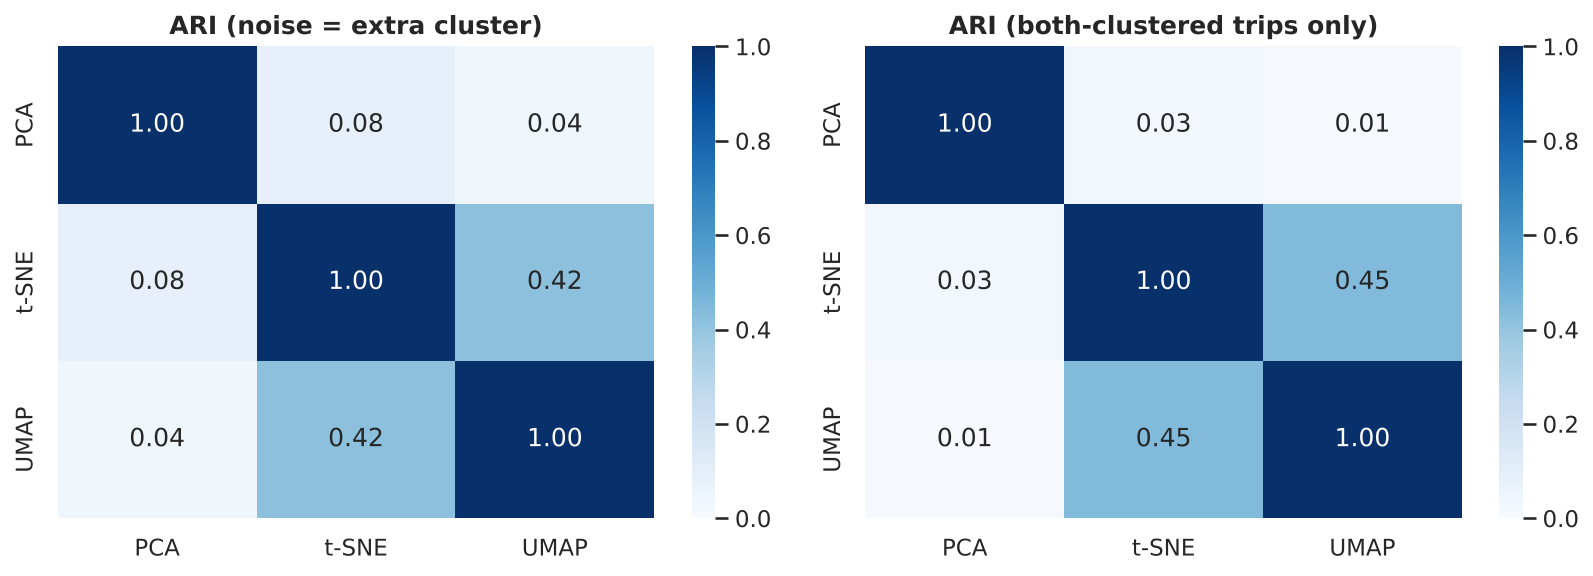
\includegraphics[width=0.6\linewidth]{q6_6_ari}\caption{Adjusted Rand index between the three clusterings.}\end{figure}

\textbf{Recommendation.} For exploring this data set we recommend \textbf{UMAP as the primary tool} (small $\text{min\_dist}$, $n_\text{neighbors}\approx15$--50), \textbf{PCA alongside} for interpretable axes, and t-SNE only as a cross-check. UMAP was several times faster than t-SNE, more stable across seeds in our test (ARI 0.86--0.90 against 0.39--0.85 for random-initialisation t-SNE), nearly as locally faithful (0.96 vs 0.98) with comparable global fidelity, and its separated islands make density-based clustering straightforward. PCA is deterministic and instantaneous, shows that eight dimensions are needed for 90\,\% of the variance and has readable loadings; every cluster found in UMAP or t-SNE should still be profiled in the original feature space. A caveat on our own results: the seven day-of-week islands arise largely because day of week is a discrete feature in the feature matrix; encoding it as a weekend flag (or omitting it) would remove them and emphasise location, distance and speed.

\section*{Conclusions}
The cleaned data (98.6\,\% of trips) show a clear weekly rhythm: Friday/Saturday are busiest, weekdays are commute-driven (peaks 18:00--21:00) and weekends nightlife-driven; only Memorial Day alters the daily volume. The spatial pattern is a residential-to-business flow in the morning, the reverse in the evening, and downtown nightlife at weekends; taxi hotspots are compact street corners that differ between Friday night and Thursday evening. Trips from the Empire State Building take about 46 min to JFK and 33 min to Newark, with a strong afternoon penalty. Dimensionality reduction shows that the data are high-dimensional (8 PCs for 90\,\%); the non-linear methods expose the day-of-week and airport structure, but their clusters, distances and sizes must be validated rather than read at face value.

\appendix
\section{Pickup locations of the PCA and t-SNE clusters}
The pickup locations of the largest clusters (and of the airport-dominated clusters) of the PCA and t-SNE clusterings of Section~6.5 are shown below in the same way as the UMAP clusters in Figure~\ref{fig:maps} (red = the cluster's pickups, grey = all sampled pickups). The cluster profiles of all clusters are printed in the notebook. As for UMAP, the large clusters (one giant cluster for PCA; day- and time-of-day groups for t-SNE) cover the same Manhattan footprint. The airport clusters have their pickups either at an airport (LaGuardia or JFK) or in Manhattan (trips towards the airport).
\begin{figure}[!htbp]\centering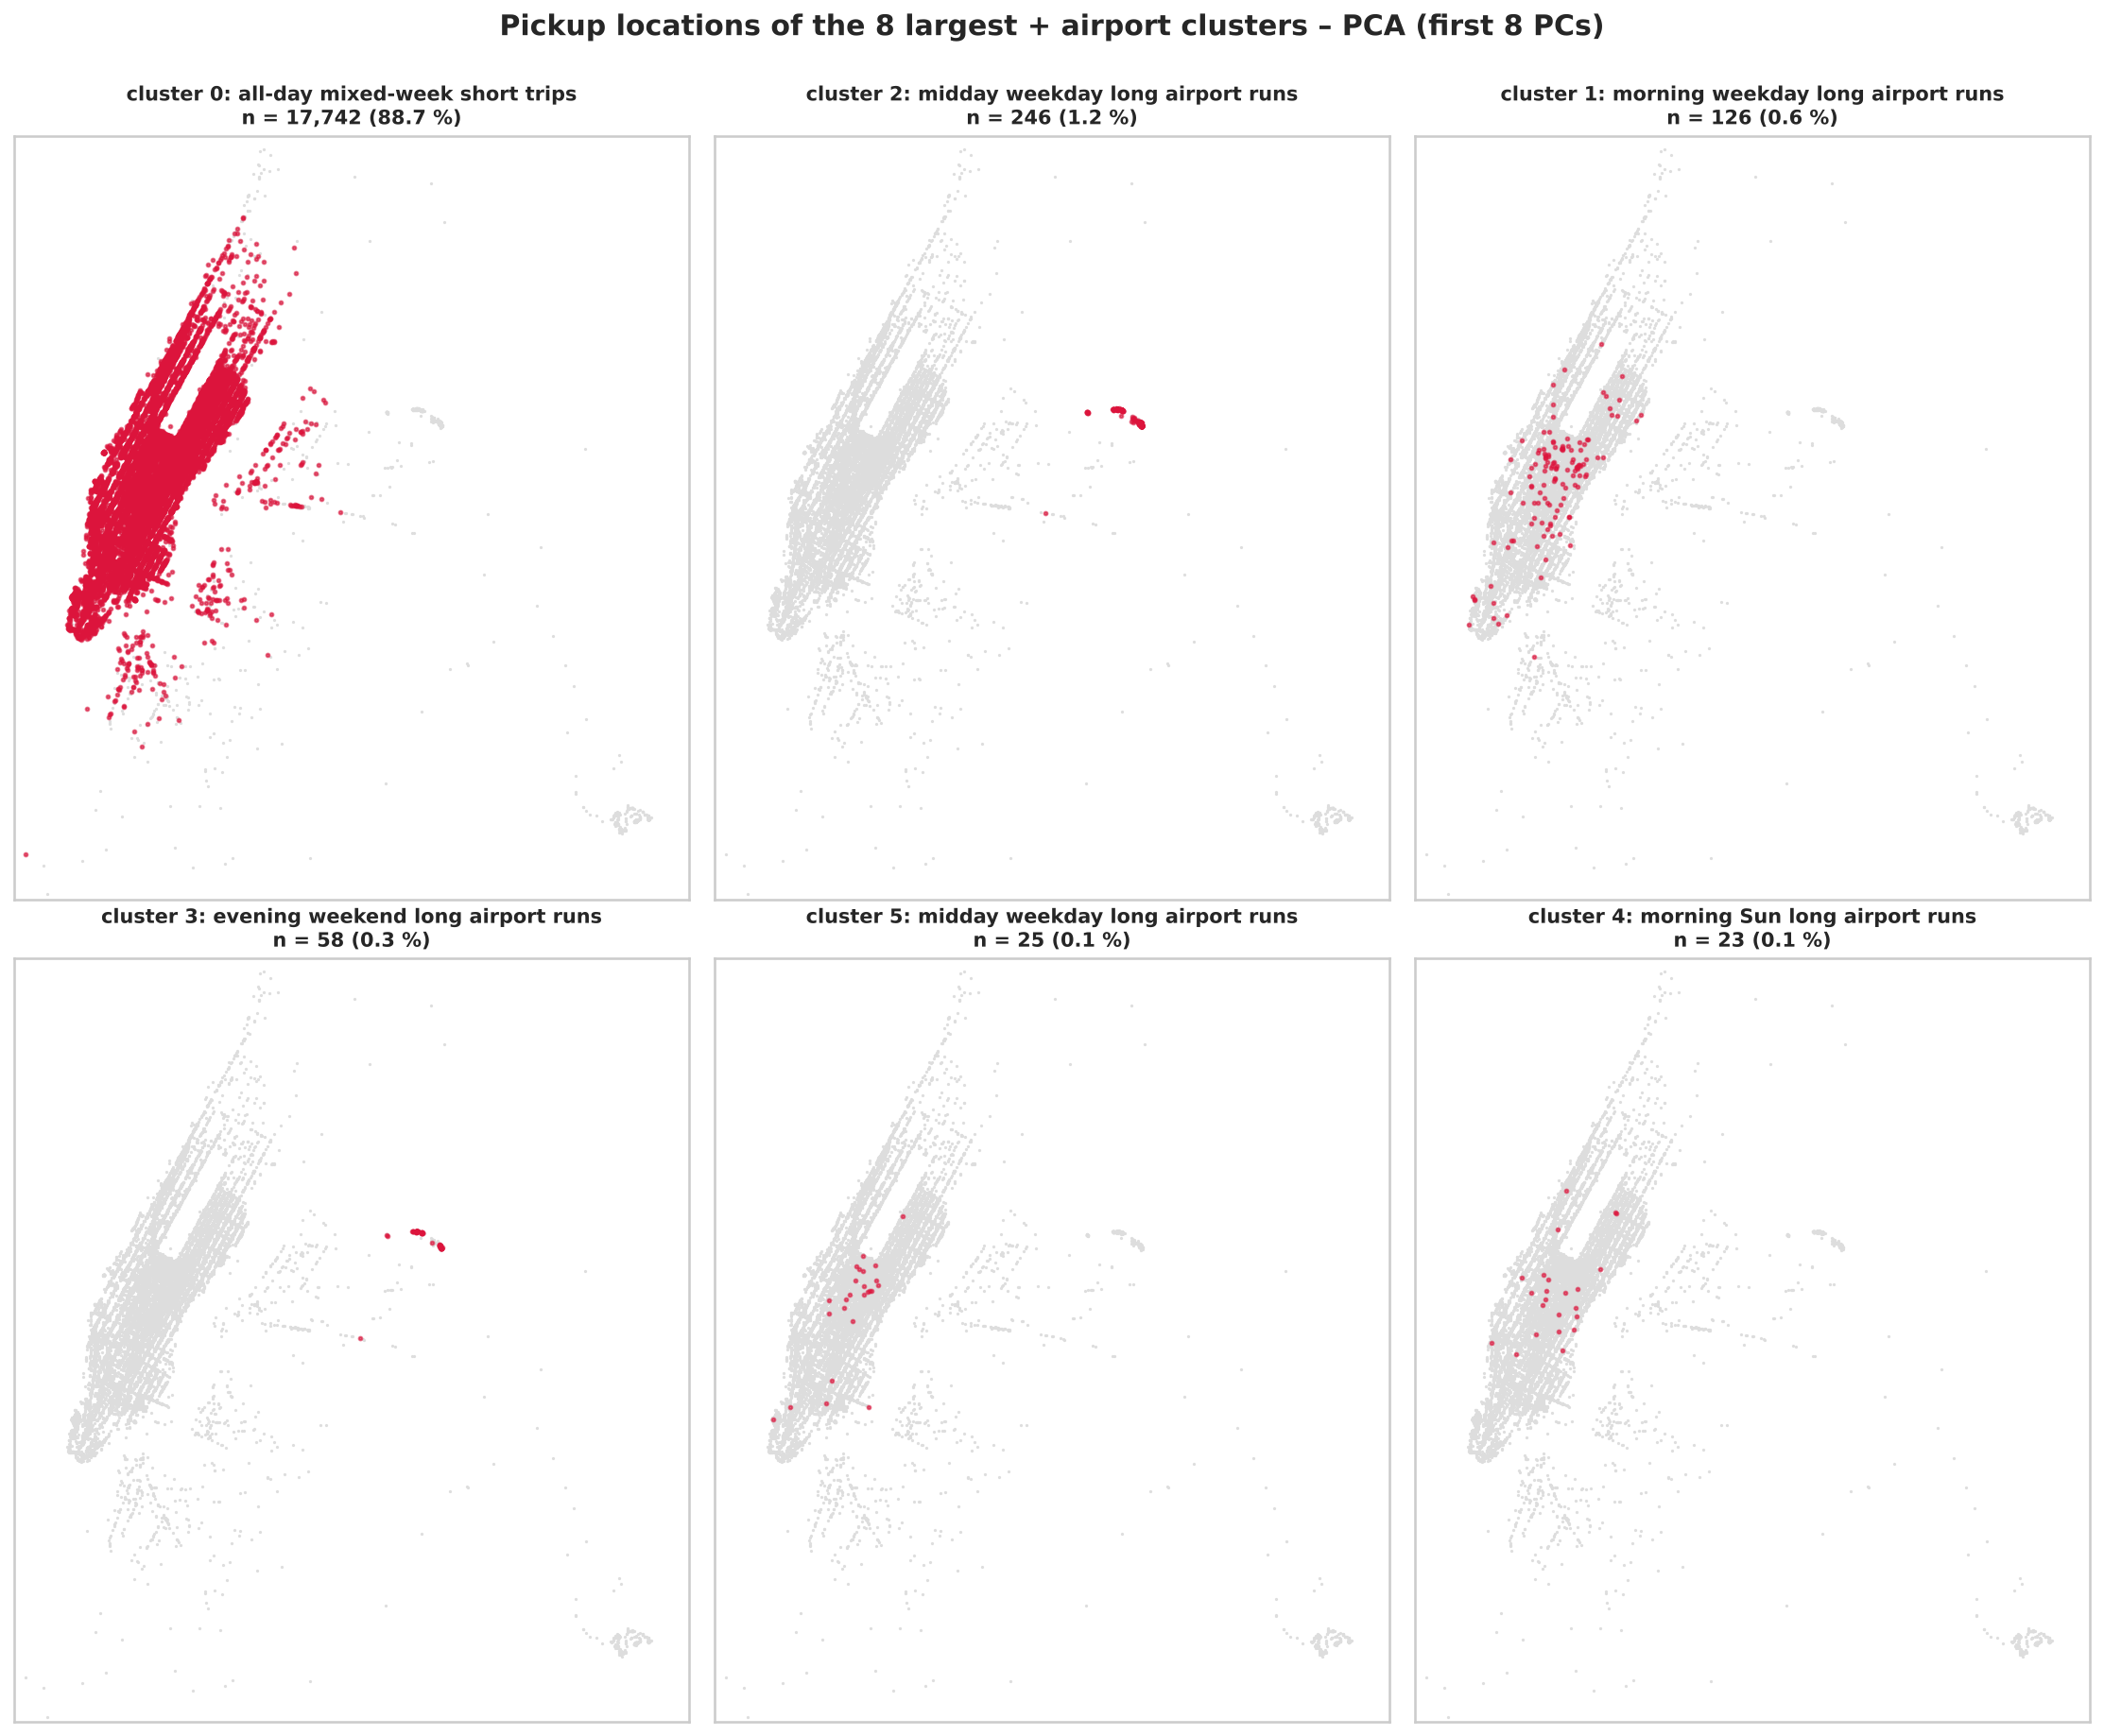
\includegraphics[width=0.95\linewidth]{q6_5_maps_pca}\caption{PCA (first 8 components) clusters: pickup locations of the largest and the airport-dominated clusters.}\label{fig:mapspca}\end{figure}
\begin{figure}[!htbp]\centering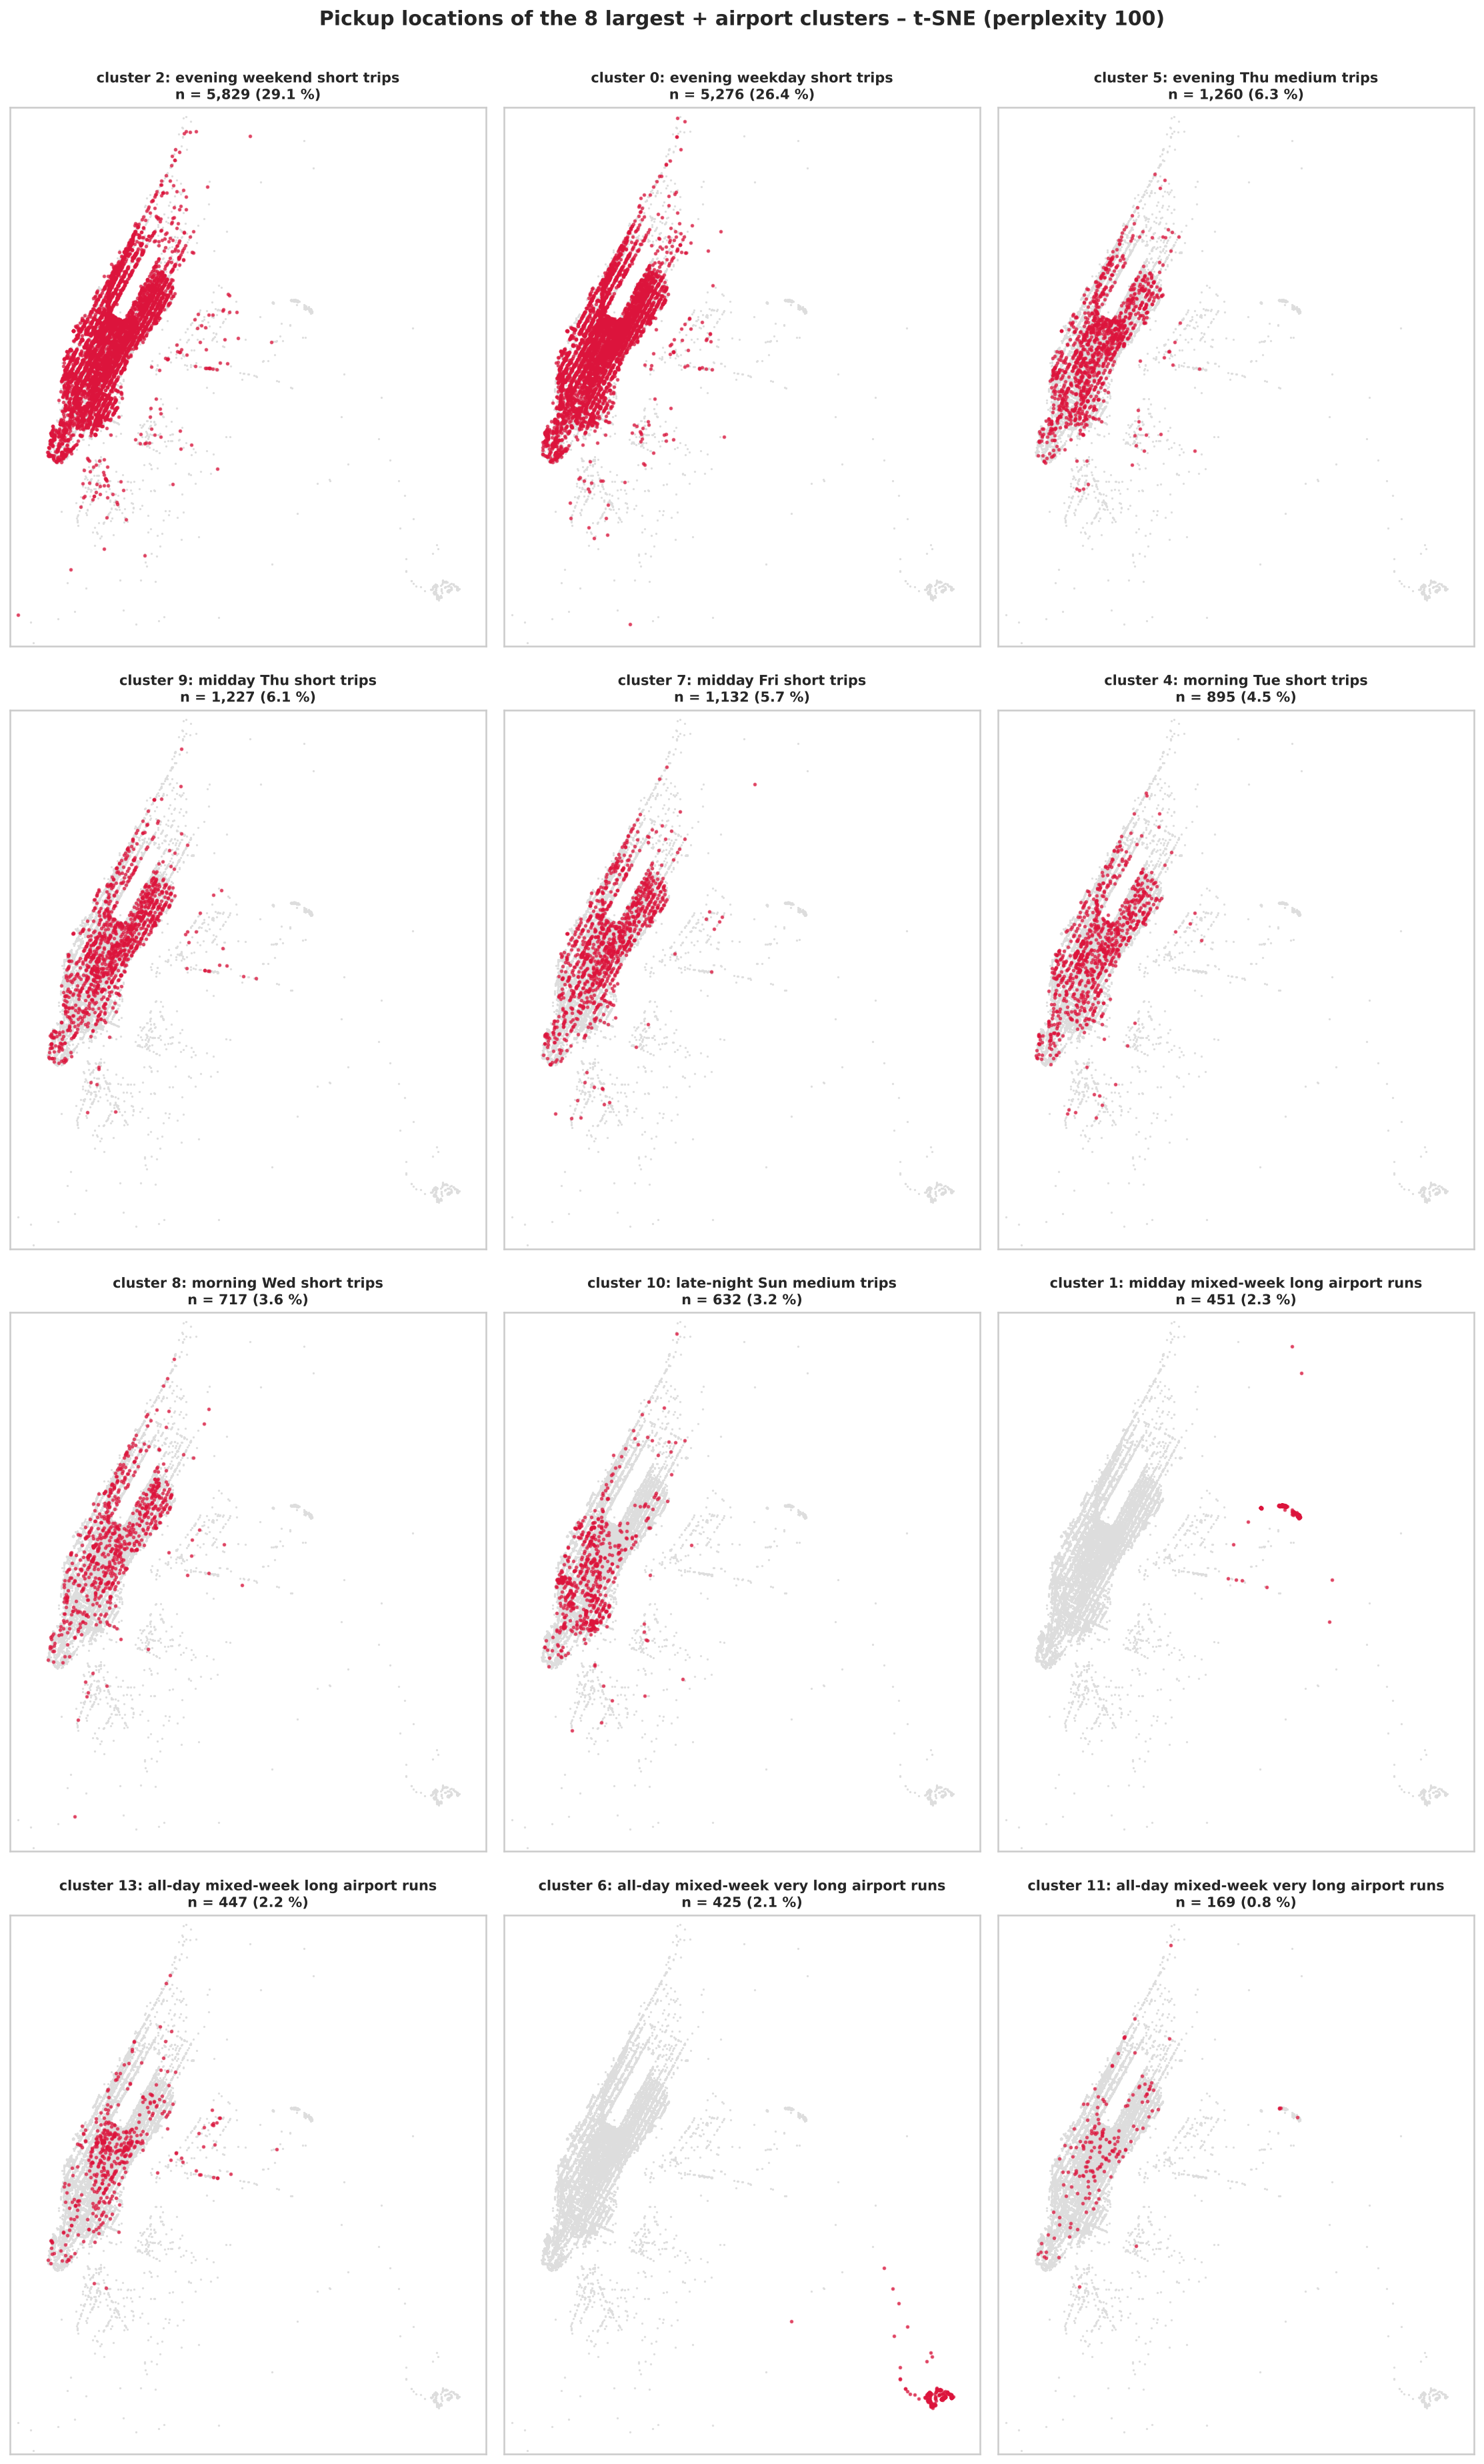
\includegraphics[width=0.74\linewidth]{q6_5_maps_tsne}\caption{t-SNE (perplexity 100) clusters: pickup locations of the eight largest and the airport-dominated clusters.}\label{fig:mapstsne}\end{figure}

\end{document}
